\documentclass[11pt,letterpaper]{article}

\usepackage[T1]{fontenc}
\usepackage{lmodern}
\usepackage{microtype}
\usepackage[margin=1in]{geometry}
\linespread{1.0}
\setlength{\parskip}{0pt}          % conventional article: indent, no vertical gap
\setlength{\parindent}{1.5em}

\usepackage{amsmath,amssymb,amsthm}
\usepackage{graphicx}
\usepackage{xcolor}
\usepackage{tikz}
\usepackage{booktabs,tabularx,array,longtable}
\newcolumntype{L}[1]{>{\raggedright\arraybackslash}p{#1}}
\usepackage{listings}
\lstset{basicstyle=\ttfamily\footnotesize,breaklines=true,columns=fullflexible,frame=single,framesep=4pt,showstringspaces=false,captionpos=b}
\usepackage[hidelinks]{hyperref}
\usepackage{cleveref}

\newtheorem{theorem}{Theorem}[section]
\newtheorem{proposition}[theorem]{Proposition}
\newtheorem{lemma}[theorem]{Lemma}
\newtheorem{corollary}[theorem]{Corollary}
\theoremstyle{definition}
\newtheorem{definition}[theorem]{Definition}
\newtheorem{assumption}[theorem]{Assumption}
\newtheorem{example}[theorem]{Example}
\theoremstyle{remark}
\newtheorem{remark}[theorem]{Remark}

\usetikzlibrary{arrows.meta,positioning}
\usepackage{everypage}
\definecolor{grokgray}{RGB}{110,110,110}
\AddEverypageHook{%
  \ifnum\value{page}=1
    \begin{tikzpicture}[remember picture, overlay]
      \node[rotate=90, anchor=south, font=\footnotesize\sffamily\color{grokgray}, inner sep=0pt]
        at ([xshift=30pt, yshift=0.5\paperheight]current page.south west)
        {GrokRxiv:2026.10.transaction-log-source-control\quad [\,cs.DC\,]\quad 20 Oct 2026};
    \end{tikzpicture}
  \fi
}


\newcommand{\R}{\mathsf{R}}
\newcommand{\W}{\mathsf{W}}
\newcommand{\Snap}[1]{S_{#1}}
\newcommand{\Log}{\mathcal{L}}
\newcommand{\Loc}{\mathcal{T}}
\newcommand{\meets}{\bowtie}
\newcommand{\nmeets}{\not\bowtie}
\newcommand{\cov}{\sqsubseteq}
\newcommand{\Later}{\mathrm{Later}}
\newcommand{\tree}{\tau}
\newcommand{\fp}{\pi_1}
\DeclareUrlCommand\code{\def\UrlFont{\ttfamily\small}}
\newcommand{\mcode}[1]{\text{\texttt{\small #1}}}
\makeatletter\g@addto@macro\UrlBreaks{\do\_\do\#\do\:}\makeatother

\title{A Transaction Log for Source Control\\[4pt]
  {\normalsize Part I of \emph{Source Code as a Transactional Abstraction}}}
\author{Matthew Long\\
  \small The YonedaAI Collaboration, YonedaAI Research Collective\\
  \small Chicago, IL\\
  \small \texttt{matthew@yonedaai.com} \textperiodcentered\ \url{https://yonedaai.com}}
\date{October 2026}

\begin{document}
\maketitle

\begin{abstract}
Source code and source control can now be treated as transactional abstractions: a repository is a database, a change is a transaction with a read set and a write set, landing is a commit under optimistic concurrency, and a version is a snapshot. This paper gives the transaction model on which that view rests. In Git, when many always-online agents write against one moving branch, every lost compare-and-swap race on the branch costs a rebase, a retest and a retry. In the model, commits are built on the server and recorded without moving any ref. A landing validates the change against every log entry written since its base and appends one hash-chained entry in the same atomic step as the ref update, performed by a serialized authority per repository. We prove replay determinism, snapshot immutability, refs that advance only along first-parent chains, and serializability, relative to declared read sets, of landings that need no line-level merge. The companion paper's independence condition is exactly the condition under which two changes land without merging in either order. The model's known gap is in group landing: a combiner that validates batch members only against the log admits write skew between them, and we give the check that removes it. In a reference implementation, the merge matched \texttt{git merge-file} on 300 of 300 random merges, and a changeset landing path landed 1,000 of 1,000 concurrent writers in each of six hosted bursts; a sustained landing rate remains unmeasured. % M65, M220, M221
\end{abstract}

\section{Introduction}
\label{sec:tlsc:intro}

Source code and source control are now transactional abstractions. A repository is a database whose state is a set of refs over immutable objects. A change is a transaction that reads part of the source and writes another part. Landing a change is a commit under optimistic concurrency control, and a version of the repository is a snapshot. This paper lays the base layer of that view: a transaction model for source control, with its log, its snapshots, its isolation level, its validation rule and its serializability guarantee, together with the place where the implemented system falls short of the model.

We argue that this is the next step in how code is managed, and that data took the same step first. Data lakes began as files on object stores; concurrent writers and derived computation broke file-level semantics, and the field moved to tables with a transaction log, snapshots and optimistic concurrency \cite{armbrust2020delta,icebergspec}, with partitioned computation running over those snapshots \cite{zaharia2012rdd}. Agents now put source control under the same pressure, by multiplying concurrent writers and the volume of derived work. Scion's published design makes the same move: it creates changesets on the server as entries in a write-ahead log and keeps the ref update as a compare-and-swap on one database row, separate from commit creation \cite{anthropic2026scion}. This series supplies foundations for that move, and the proofs and measurements of Parts I to III are the evidence for the thesis.

Source control was designed for people. A developer clones a repository, edits files on a local disk, builds a commit, and pushes it. The server sees a finished commit and one request to move a branch from an old value to a new one. If the branch moved in the meantime, the push is refused and the developer fetches, rebases, retests and tries again. This loop is cheap when conflicts are rare and the writer is patient. It is expensive when writers are numerous, short-lived and always online, and when each of them writes a few files against the same branch head.

That situation now exists. Anthropic reports that its merge rate grew from about 2,500 code changes per day in May 2026 to more than 30,000 per day by September, and that git traffic, mirror drift and merge coordination became its largest development bottleneck \cite{anthropic2026scion}. % S-1, S-2
Its response, a system called Scion, replaces commits created on clients with changesets created on the server as entries in a write-ahead log, and moves a ref by a compare-and-swap on a single database row that is not involved in creating or fetching commits \cite{anthropic2026scion}. % S-14

This paper studies the same problem from the side of data systems. We treat a repository the way Delta Lake treats a table \cite{armbrust2020delta}. Immutable objects play the role of data files. An append-only, hash-chained transaction log records every ref change. Checkpoints summarize the log so that any version can be reconstructed cheaply. Readers pin a version and see a snapshot. Writers validate optimistically against what has been committed since they read. The analogy is close enough to transfer the main correctness arguments, and it fails in two places that matter: the snapshot of a repository is a map of refs, not a set of files, and two writers that touch the same file can often both succeed through a three-way merge, which has no counterpart in a table.

The architecture needs four primitives: an immutable, content-addressed object store; a serialized authority per repository that holds durable state and executes each command atomically; a durable queue with retries; and stateless compute. The log, the refs and the validation logic live in the serialized authority, which supplies the atomic step that Delta Lake obtains from put-if-absent writes to an object store \cite{armbrust2020delta}. Every theorem in this paper is stated over these primitives. Scion's ref update, a compare-and-swap on one Spanner row \cite{anthropic2026scion,corbett2012spanner}, shows that a serialized authority of this kind is available outside the platform we used.

The reference implementation, YonedaRepo, is first-party work: the author designed and built it. It offers Git semantics (commits, branches, merges, diffs and logs) with Git object identifiers, so every commit it exposes can be fetched and verified by stock Git. It realizes the primitives on Cloudflare, with a Durable Object as the serialized authority \cite{cfdoconcepts,cfdosqlite}; Part III gives the mapping of each primitive to a product and the measured cost of the authority (Part III, Sections~3, 5 and~6) \cite{long2026partIII}. Part II describes derived data as views maintained from the log \cite{long2026partII}.

The paper makes five contributions.
\begin{enumerate}
\item A formal model of a source repository as a transaction log over content-addressed Git objects, with snapshots, checkpoints and time travel by version or commit (Section~\ref{sec:tlsc:framework}).
\item Proofs that replay is deterministic, that snapshots are immutable, that refs only advance along first-parent chains in the implemented system, and that no landed change is lost (Section~\ref{sec:tlsc:log}).
\item A serializability theorem for landings validated against declared read sets, with a mapping to the validation conditions of Kung and Robinson \cite{kung1981occ}, and an exact characterization of the companion paper's independence condition (Eq.~1 of \cite{long2026inversion}) as the condition for order-insensitive landing without a merge (Section~\ref{sec:tlsc:occ}).
\item An analysis of the group-landing combiner that proves it preserves the single-writer property of the ref update, shows by counterexample that it admits write skew between members of one batch, and gives a sufficient condition that removes the anomaly (Section~\ref{sec:tlsc:combiner}).
\item A statement of the intended changeset landing path, in which the Git commit of a branch is a deterministic function of the log prefix, and a check of which results carry over to it unchanged (Section~\ref{sec:tlsc:n11proof}).
\end{enumerate}
The measured evidence in Section~\ref{sec:tlsc:evidence} is correctness evidence first: Git object identity, agreement of the merge with Git, and concurrent landings without loss. The hosted latency of the write path misses its design target, and we say so there.

\section{The coordination problem}
\label{sec:tlsc:problem}

\subsection{Git's unit of coordination}

Git names every object by the SHA-1 digest of a short header and the object's bytes \cite{gitobjects}. A commit names one tree and its parents; a tree names blobs and subtrees. The naming makes objects immutable and verifiable by anyone who holds them, which is the property every later design keeps.

Coordination in Git happens at refs. A push sends, for each ref, a command with the old and new object identifiers, followed by a pack of objects; the server unpacks the objects, checks that each ref still has the old value the client named, and updates it \cite{gitprotocol}. The ref update is therefore a compare-and-swap. Everything before it, including building the commit, computing which objects the server lacks and producing the pack, happens on the client. When the swap fails, all of that work is stale. The client must fetch the new head, rebuild its commit on top of it, rerun whatever checks it trusts, and push again.

For a person, this loop is a minor tax. For a large population of writers that share a branch, the loop becomes the system. Each failed swap converts into a fetch, a rebase and a retry, and the probability of failing grows with the rate at which others land. The cost of a lost race is paid on the client, where the writer cannot see what else is happening, and it is paid in full even when the competing change touched unrelated files.

\subsection{Always-online writers}

An agent that edits code differs from a person in three ways that matter here. It is always online, so it does not need an offline copy of history. It is short-lived, so a full clone is mostly wasted work. It usually changes a few files and could tell the server what it read and what it wrote. None of these facts is exploited by the push protocol, which assumes that the client holds the history and the server holds only the result.

The Scion post quantifies the consequences at one company: a main-branch history of almost 100 GB, compressed working copies over 25 GB, on the order of 25 million CI checkouts per day, and an estimated 600 PB per day of git traffic if every checkout fetched naively \cite{anthropic2026scion}. % S-3, S-4, S-5, S-6
Several hundred git mirrors were needed to carry the load, and their seeds drifted from the main branch between refreshes \cite{anthropic2026scion}. % S-7
The post also argues that a strict merge queue does not suit agent-scale merging, because many changes land while any one change is being tested \cite{anthropic2026scion}. These are reported figures from one organization's production system. We use them as motivation, not as measurements of the system studied here.

\subsection{Requirements}

From these observations we draw five requirements for a replacement processing model. They are design requirements, not empirical claims.
\begin{description}
\item[D1, server-side changes.] A writer sends file changes and receives a commit identifier. The server builds trees and commits and stores the objects.
\item[D2, creation separate from landing.] Creating a commit must not move a ref, so that commits can be created in parallel without coordination and checked before they land.
\item[D3, cheap lost races.] When the branch moved, the server should decide from recorded metadata whether the change still holds, and merge it without a client round trip when it does.
\item[D4, contention-free reads.] Reads should name an immutable version and never wait for writers.
\item[D5, Git semantics.] Writers and readers should see commits, branches, merges, diffs and logs with Git's meaning, and a branch should be exportable as Git objects that existing tools can fetch and verify.
\end{description}
Scion meets D1 to D4 with its own changeset format and describes itself as not a general Git replacement \cite{anthropic2026scion}. The design here meets D1 to D4 with the log described below. D5 constrains what the log must be able to produce, not what a landing must write: the Git objects of a branch can be built from the log, as Section~\ref{sec:tlsc:n11} explains.

\section{Design}
\label{sec:tlsc:components}

The design has four components, each built on the primitives named in the introduction. Table~\ref{tab:tlsc:components} compares each with its counterpart in Scion. Part III maps the primitives to products in the reference implementation.

\begin{table}[t]
\centering
\small
\caption{The four components. Scion's column paraphrases the Scion post \cite{anthropic2026scion}.}
\label{tab:tlsc:components}
\begin{tabularx}{\textwidth}{@{}L{2.4cm}XX@{}}
\toprule
Component & Scion & This architecture \\
\midrule
Objects & Content-addressed compressed blobs in cloud storage behind cache tiers & Git blobs, trees and commits in an object store, read through caches keyed by object identifier \\
Workspace changesets & Write-ahead log entries listing files changed against the first parent & Commits built and recorded by the authority, with their changed paths, before any ref moves \\
Protected refs & A compare-and-swap on one Spanner row per ref & Refs and one transaction log per repository in the serialized authority \\
Compute & Server-side services for merge, derived data and checks & Stateless functions for merge, rewrite and search, container compute for checks, and a durable queue for follow-up work \\
\bottomrule
\end{tabularx}
\end{table}

\subsection{Objects}

Objects are Git objects with Git identifiers. The platform computes the identifier of a blob, tree or commit as the SHA-1 of the header \texttt{\small <type> <size>\textbackslash 0} followed by the bytes, the same rule Git uses \cite{gitobjects}, and its codec reproduces identifiers that Git itself computes with \code{hash-object}, \code{mktree} and \code{commit-tree} (Appendix~\ref{app:tlsc:evidence}). Packs sent to the object store contain only whole objects; the reader refuses deltified entries.

In the reference implementation at \code{cfa4845}, Git objects live in a Cloudflare Artifacts repository, with R2 and an edge cache as read-through tiers. Later revisions of the development branch make R2 the store of record and push only protected refs to Artifacts (Part III, Section~3.2).

Every recorded commit is kept reachable in the object store by a hidden ref named after the commit, so that work which no branch points at yet cannot be collected. The only maintenance the platform performs is releasing these hidden refs once a commit is safely reachable from a branch or once unlanded work has expired; Part II analyzes that procedure in its Proposition~12.1.

\subsection{Workspace changesets}

A writer sends a list of file changes, a parent commit, a base log version, an optional declared read set and a message. The authority computes the new tree by rewriting only the directories on changed paths, asks the adapter for exactly the existing trees it needs, verifies every supplied tree against its identifier, and returns the objects to upload. After the adapter has pushed the objects and read the commit back from the object store, the authority records it. A recorded commit carries its tree, its parents, its base version, its read set and its list of changed paths relative to the first parent. In the words of the code, it is durable, addressable work that no ref points at yet.

The rewrite gives the scaling property Scion asks for: the number of trees read and written depends on the directories along the changed paths, not on the number of files in the repository. Proposition~\ref{prop:tlsc:rewrite} states this precisely.

\subsection{Protected refs}

Refs live in one table inside the repository's serialized authority, next to the transaction log, the checkpoints, the land queue and the table of landings. A landing is one call into the authority. The call reads the ref, validates the change against the log, and either refuses or appends one log entry and updates the ref, all as one atomic command. The contract the design needs from the authority is that its commands behave as if executed one at a time, each committing all of its writes or none. No network input or output happens inside a command: object pushes and reads happen in the adapter before the authority is called. These two properties are the basis of the formal model in Section~\ref{sec:tlsc:framework}. The reference implementation obtains them from a Durable Object, which runs one request at a time and whose synchronous SQLite transactions are all-or-nothing \cite{cfdoconcepts,cfdosqlite}. A transactional database that offers serializable transactions over the ref row and the log tail would provide the same contract.

The design deviates from Scion in one respect that matters for capacity. Scion places each ref on its own database row \cite{anthropic2026scion}. This architecture places all refs of a repository, and the preparation and recording of every commit, behind one authority. Serialization is therefore per repository, not per ref. That is a choice of key for the authority, not a property of the primitive, and a realization could key authorities by ref instead. Part III measures the consequences in its Sections~4 to~6.

\subsection{Compute}

Diffs, three-way merges, tree rewrites, symbol extraction and search run as stateless functions called from the adapter; in the reference implementation they are Rust compiled to WebAssembly and run in Workers. Checks run in container compute on the exact commit they certify. A durable queue carries derived-data jobs and ref projection to the Git-facing store. None of these components holds authority: their outputs are either content-addressed objects, which anyone can verify by hashing, or proposals that the authority verifies before it accepts them.

\begin{figure}[t]
\centering
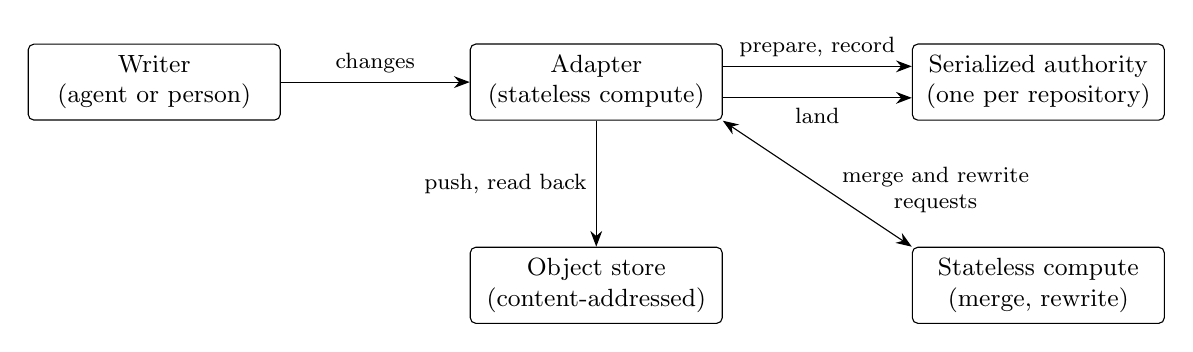
\begin{tikzpicture}[
  box/.style={draw, rounded corners=2pt, align=center, font=\small, minimum height=9mm, minimum width=3.2cm, inner sep=4pt},
  lab/.style={font=\footnotesize, align=center},
  >={Stealth[length=2mm]}]
\node[box] (client) {Writer\\(agent or person)};
\node[box, right=2.4cm of client] (worker) {Adapter\\(stateless compute)};
\node[box, right=2.4cm of worker] (auth) {Serialized authority\\(one per repository)};
\node[box, below=1.6cm of worker] (store) {Object store\\(content-addressed)};
\node[box, below=1.6cm of auth] (compute) {Stateless compute\\(merge, rewrite)};
\draw[->] (client) -- node[lab, above] {changes} (worker);
\draw[->] ([yshift=2mm]worker.east) -- node[lab, above] {prepare, record} ([yshift=2mm]auth.west);
\draw[->] ([yshift=-2mm]worker.east) -- node[lab, below] {land} ([yshift=-2mm]auth.west);
\draw[->] (worker) -- node[lab, left] {push, read back} (store);
\draw[<->] (worker.south east) -- node[lab, pos=0.55, right=2pt] {merge and rewrite\\requests} (compute.north west);
\end{tikzpicture}
\caption{The write path. Creating a commit (prepare, push, read back, record) and landing it are separate calls. Only the land call reads and updates refs, and it performs no network input or output while it holds the authority's transaction.}
\label{fig:tlsc:path}
\end{figure}

\subsection{Commit creation and ref moves}

Figure~\ref{fig:tlsc:path} shows the separation that requirement D2 asks for. A commit is created by four steps that never touch a ref: prepare, push, read back and record. Reviews and check results attach to the commit identifier. Landing is a fifth, separate step. Its gates require the configured approvals and passing results for the required checks, bound to the policy in force; a change whose every file falls in a class the policy marks safe, such as comments only, counts as approved, and an unclassified change never does. Landing then validates and appends. If the branch moved and the change needs a merge, the platform builds a merge commit with its own compute, records it under the principal \code{platform:merge}, and lands that merge in place of the original commit. Original commit identifiers are never rewritten.

\subsection{Realizations of landing}
\label{sec:tlsc:n11}

The reference implementation first landed commits: every landing that is not a fast-forward builds a platform merge commit, with new tree objects on every changed path, before the authority appends the entry. This tree-building landing is the path the code evidence of Sections~\ref{sec:tlsc:framework} to~\ref{sec:tlsc:combiner} describes, at revision \code{cfa4845}, and it was still the landing path of the development branch at revision \code{03821e0}. Building Git objects on the landing path is a choice of that implementation, not a requirement of D5.

The architecture's intended landing path lands changesets instead. It was first implemented and measured at revision \code{dd6c9a8} on the branch \code{claude/native-p95e}, and it is merged into the development branch at revision \code{fef94e7}. A landing carries a base version, a declared read set and a list of file changes. The authority validates it by path overlap against the log entries since its base, which is a query on the log, and appends one entry; many landings share one authority command. Two paths result. When the changeset's paths are disjoint from every later entry's paths, landing is the validation query and the append, with no file content read. When a later entry wrote one of the same files, landing takes the merge path, which reads the three versions of each shared file and runs the three-way merge. The Git commit of the branch is built afterwards, in the background, as a deterministic function of the log prefix: the same prefix always yields the same commit identifier. Part II treats that projection as a derived view of the log. The cost is that a branch's Git identifier becomes available after its landing returns rather than with it. At \code{fef94e7}, 1,000 of 1,000 concurrent writers landed in each of six hosted bursts on the reference implementation. % M220, M221
Part III reports its latency and throughput.

Every result of Sections~\ref{sec:tlsc:log} to~\ref{sec:tlsc:combiner} is stated over log entries, read sets, write sets and validation outcomes. Section~\ref{sec:tlsc:n11proof} checks which of them carry over to changeset landing unchanged and which become properties of the projection.

\section{Mathematical framework}
\label{sec:tlsc:framework}

This section states the model. Each definition corresponds to a data structure or function in the implementation; Appendix~\ref{app:tlsc:evidence} gives the file and commit for each.

\subsection{Objects, trees and commits}

\begin{definition}[Object store]
\label{def:tlsc:objects}
Let $\mathit{Id}$ be the set of 160-bit identifiers. An \emph{object store} is a finite partial map $O:\mathit{Id}\rightharpoonup\mathit{Type}\times\mathit{Bytes}$, with $\mathit{Type}=\{\mathrm{blob},\mathrm{tree},\mathrm{commit},\mathrm{tag}\}$, such that $O(x)=(k,b)$ implies $x=H(\mathit{hdr}(k,b)\,\|\,b)$, where $H$ is SHA-1 and $\mathit{hdr}(k,b)$ is Git's header naming the type $k$ and the length of $b$. The store only grows: if $O\subseteq O'$ describes two moments in time, every object of $O$ is in $O'$ with the same type and bytes.
\end{definition}

Content addressing makes an object immutable by construction. Two stores that hold an identifier hold the same bytes, unless $H$ has a collision. All results below assume that no collision occurs among the objects of one repository; Git makes the same assumption, and its hash transition to SHA-256 would weaken it further without changing any argument here.

A \emph{tree state} $\tree$ is a finite map from file paths to blob identifiers and modes, the decoded form of a Git root tree. A \emph{commit} $c$ has a tree state $\tree(c)$ and a list of parents; $\fp(c)$ is its first parent, or $\bot$ for a root commit. Every recorded commit also has a \emph{generation} one greater than the largest generation of its parents, so the parent relation is acyclic.

\begin{definition}[Touched paths]
\label{def:tlsc:touched}
The \emph{change} of a commit $c$ is the set $\Delta(c)$ of paths whose entry differs between $\tree(c)$ and $\tree(\fp(c))$, with every path of $\tree(c)$ counted when $\fp(c)=\bot$. The platform records with $c$ a set $T(c)$ of \emph{touched paths}, viewed as file nodes of the location tree of Definition~\ref{def:tlsc:access}; alongside each it stores an operation (add, modify or delete) and the old and new blob, which the results below do not use.
\end{definition}

The authority derives $T(c)$ from the change list it was given and builds $\tree(c)$ by applying exactly that list to $\tree(\fp(c))$. Hence $\Delta(c)\subseteq T(c)$ for every commit the platform prepares, including the merge commits the platform builds when landing work on a moved branch: the adapter submits each of them to the same preparation command, with the head as first parent and the merged commits as further parents. A property test checks that the incremental rewrite produces the same tree as building it from scratch.

\begin{proposition}[Rewrite cost]
\label{prop:tlsc:rewrite}
Let $c$ change the set of paths $P$ relative to $\fp(c)$, and let $D(P)$ be the set of directories that are proper prefixes of some path in $P$, including the root. Preparing $c$ reads exactly the trees of $D(P)$ that exist in $\tree(\fp(c))$ and encodes exactly the trees of $D(P)$ that are non-empty in $\tree(c)$; a directory left empty is removed from its parent instead. The work is $O\bigl(\sum_{d\in D(P)}|d|\bigr)$, where $|d|$ is the number of entries of directory $d$ in $\tree(\fp(c))$ and $\tree(c)$ together, and is independent of the number of files outside $D(P)$.
\end{proposition}

\begin{proof}
A tree's identifier depends only on its entries. A directory not in $D(P)$ contains no changed path, so its entries and hence its identifier are unchanged, and its parent can reuse the identifier without reading it. A directory in $D(P)$ contains a changed path, so at least one entry changes and the directory must be re-encoded, which requires reading its existing entries. Re-encoding a directory costs time linear in its entries. Summing over $D(P)$ gives the bound.
\end{proof}

The bound depends on directory fan-out, so a flat directory of many files makes a one-file change expensive. It does not depend on repository size as such. The unit test \code{rewriting_reads_only_directories_on_changed_paths} checks that an unchanged subtree is never read.

\subsection{Locations and access sets}

Read and write sets name parts of the source at two granularities: files and directory prefixes, and symbols inside files. We model both as nodes of one tree.

\begin{definition}[Location tree and overlap]
\label{def:tlsc:access}
The \emph{location tree} $\Loc$ is the rooted tree of all syntactically valid locations, whether or not a given tree state contains them. Its nodes are the root, directories, files and symbols; a directory's children are the directories and files named inside it, a file's children are its top-level symbols, and a symbol's children are its nested members. An \emph{access} is a node of $\Loc$. Write $a\cov b$ when $a$ is an ancestor of $b$ or equal to it. Two accesses \emph{overlap}, written $a\meets b$, when $a\cov b$ or $b\cov a$. For sets of accesses, $X\meets Y$ holds when some $x\in X$ and $y\in Y$ overlap, and $X\nmeets Y$ otherwise.
\end{definition}

In the implementation, an access is a string: a path such as \code{src/lib.rs}, a prefix such as \code{src/}, or a symbol entry such as \code{src/lib.rs#Policy::backoff}. Two paths overlap when they are equal or when one is a prefix of the other at a component boundary, so \code{src/a} and \code{src/ab} do not overlap. Two symbol entries overlap when they name the same file and one symbol path is a \code{::} prefix of the other. A path and a symbol overlap when the path overlaps the symbol's file. The code adds one further case, for files whose literal names contain \code{#}, which can only add overlaps. The implemented relation therefore contains the relation of Definition~\ref{def:tlsc:access}. Extra overlaps are the safe direction for the soundness results below, which can only gain conflicts and merges.

\begin{lemma}[Overlap]
\label{lem:tlsc:overlap}
Let $\mathrm{sub}(a)=\{x\in\Loc : a\cov x\}$. Then $a\meets b$ if and only if $\mathrm{sub}(a)\cap\mathrm{sub}(b)\neq\varnothing$. The relation $\meets$ is reflexive and symmetric. If $a'\cov a$ and $a\meets b$, then $a'\meets b$.
\end{lemma}

\begin{proof}
If $a\cov b$ then $b$ lies in both subtrees, and symmetrically. Conversely, if $x$ lies in both subtrees then $a$ and $b$ are both ancestors of $x$; the ancestors of a node in a rooted tree form a chain, so $a$ and $b$ are comparable. Reflexivity and symmetry are immediate. For the last claim, $\mathrm{sub}(a)\subseteq\mathrm{sub}(a')$, so a common element of $\mathrm{sub}(a)$ and $\mathrm{sub}(b)$ is also in $\mathrm{sub}(a')$.
\end{proof}

Accesses are granules in the sense of multigranularity locking, where a lock on a node implicitly covers its descendants \cite[Section 3.9]{bhg1987}; overlap is intersection of that implicit coverage. We validate rather than lock, so no intention modes are needed.

\begin{definition}[Read and write sets]
\label{def:tlsc:rwsets}
A change carries a \emph{declared read set} $\R$, a finite set of accesses supplied by the writer, and a \emph{write set}. The write set of a recorded commit $c$ is $\W(c)=T(c)$ at path granularity. When the platform has parsed both sides of a touched file and found the symbols the change affected, it may replace that file by those symbols; the result is the \emph{refined} write set $\W^{\rho}(c)$. A file the platform could not resolve stays a whole-file write.
\end{definition}

A tree state assigns \emph{content} to file and symbol locations: a file's content is its blob and mode, a symbol's content is the source text the parser attributes to it, and a location the state does not contain has content $\bot$. Directories have no content of their own. Two tree states $\tree,\tree'$ \emph{agree on} a set of accesses $X$, written $\tree\equiv_X\tree'$, when they assign the same content to every file and symbol location in $\bigcup_{x\in X}\mathrm{sub}(x)$. Because absent locations have content $\bot$, agreement on a directory prefix includes agreement on which files exist below it. Agreement on a set of paths is decidable from blob identifiers alone.

\begin{definition}[Independence]
\label{def:tlsc:independence}
Two changes $i,j$ with read sets $\R_i,\R_j$ and write sets $\W_i,\W_j$ are \emph{independent} when
\begin{equation}
\W_i\nmeets(\R_j\cup\W_j)\quad\text{and}\quad\W_j\nmeets(\R_i\cup\W_i).
\label{eq:tlsc:independent}
\end{equation}
\end{definition}

Condition~\eqref{eq:tlsc:independent} is Eq.~1 of the companion paper \cite{long2026inversion}, with set intersection replaced by overlap so that a directory prefix and a file inside it count as meeting. The companion paper calls it a conservative candidate-independence condition that is only as good as the declared sets \cite{long2026inversion}. Section~\ref{sec:tlsc:eq1} makes precise what it guarantees at landing.

\subsection{The transaction log}

\begin{definition}[Log entry]
\label{def:tlsc:entry}
A \emph{log entry} is a tuple $e=(v,b,k,r,o,n,\W,\R,a,t,h)$ with version $v\geq 1$, base version $b$ with $0\leq b<v$, kind $k\in\{\mathrm{commit},\mathrm{merge},\mathrm{revert},\mathrm{import},\mathrm{ref\_move},\mathrm{ref\_delete}\}$, fully qualified ref name $r$, old and new values $o,n\in\mathit{Id}\cup\{\bot\}$, touched paths $\W$ in which no path appears twice, read set $\R$, actor $a$, commit time $t$ and chain digest $h$. Only $\mathrm{ref\_delete}$ has $n=\bot$.
\end{definition}

\begin{definition}[Hash chain]
\label{def:tlsc:chain}
Let $h_0$ be the empty string and let $\langle e\rangle$ be the canonical encoding of $e$ without its digest. The chain digest of entry $e_v$ is $h_v=G(h_{v-1},\langle e_v\rangle)$, where $G$ is SHA-256 over a canonical encoding of the pair.
\end{definition}

\begin{definition}[Log and well-formedness]
\label{def:tlsc:log}
A \emph{log} is a finite sequence $\Log=(e_1,\dots,e_n)$. It is \emph{well formed} when (I1) $e_v$ has version $v$ for every $v$; (I2) every $h_v$ equals $G(h_{v-1},\langle e_v\rangle)$; and (I3) for every $v$, the old value $o_v$ equals the value of ref $r_v$ after replaying $e_1,\dots,e_{v-1}$. The \emph{current version} of $\Log$ is $n$.
\end{definition}

The labels I1 to I3 match the invariant list in Table~\ref{tab:tlsc:invariants}. In the implementation, the log is a SQLite table keyed by version. The touched paths are copied into each entry from the commit's recorded paths at the moment of appending, so an entry is self-contained: validation never needs to consult commit metadata.

\subsection{Snapshots, replay and checkpoints}

\begin{definition}[Snapshot and replay]
\label{def:tlsc:snapshot}
A \emph{snapshot} is a finite map $S:\mathit{Ref}\rightharpoonup\mathit{Id}$. Replay applies an entry to a snapshot: $\mathrm{apply}(S,e)$ removes $r$ when $n=\bot$ and otherwise sets $r$ to $n$. For a well-formed log, $\Snap{0}=\varnothing$ and $\Snap{v}=\mathrm{apply}(\Snap{v-1},e_v)$. We call $\Snap{v}$ the snapshot at version $v$.
\end{definition}

\begin{definition}[Checkpoint]
\label{def:tlsc:checkpoint}
A \emph{checkpoint} is a triple $K=(u,S,h)$ claiming that the snapshot at version $u$ is $S$ and that the chain digest at $u$ is $h$. The implementation writes one in the same transaction as every entry whose version is a multiple of 64, stores it in the authority's database, and accepts it for a read only when $h$ equals the digest stored in the log at version $u$. % code constant, Appendix A
\end{definition}

The replay function of the implementation takes a starting checkpoint and a tail of entries. For each entry it checks that the version is the next one, that the entry is internally valid, that the recomputed chain digest matches, and that the entry's old value equals the ref's current value in the state being built; any failure aborts the read with an integrity error. This is the executable form of well-formedness.

\begin{definition}[Time travel]
\label{def:tlsc:timetravel}
A \emph{read at version} $u$, for $0\leq u\leq n$, returns $\Snap{u}$ computed by replay from the latest accepted checkpoint at or before $u$. A \emph{read at commit} $x$ returns objects reachable from $x$. A read without a version uses the ref table of the current state.
\end{definition}

Time travel works by log version and by commit identifier. A read by timestamp is not implemented: the entries carry commit times, so a timestamp could be mapped to the last version committed before it, but the read path does not do so at the commit we describe.

\subsection{The authority and its commands}

\begin{assumption}[Serialized authority]
\label{ass:tlsc:atomic}
The authority's command executions are equivalent to some sequential order of those executions. Each command runs inside one storage transaction that either commits all of its writes or none of them, and a command that returns an error commits none. No command performs network input or output inside its transaction.
\end{assumption}

Assumption~\ref{ass:tlsc:atomic} is the only property of the execution platform that the proofs use. Under it, the history of the authority's database is a sequence of committed command executions, and each command is a function from one database state to the next. The authority is then a state machine in Schneider's sense, whose deterministic commands each execute atomically with respect to the others \cite{schneider1990}. For the log, the assumption gives the contract Delta Lake states for catalog-managed tables: a catalog ``must not ratify version $v$ until it has ratified version $v-1$, and it must ratify version $v$ at most once'' \cite{deltaprotocol}.

Many stores satisfy the assumption. Any store with serializable, all-or-nothing transactions over the authority's state does. A weaker store suffices for the log alone: if appending version $n+1$ is a put-if-absent and every command re-reads the log tail it validates against, Delta's argument applies \cite{armbrust2020delta}.

The reference implementation satisfies it with a Durable Object, which processes one request at a time and whose synchronous transaction API is all-or-nothing \cite{cfdoconcepts,cfdosqlite}. The authority's dispatcher wraps every command in that API and turns any error into a rollback, and the authority's crate calls only its SQL store interface (Appendix~\ref{app:tlsc:evidence}).

\begin{definition}[Proposal and validation]
\label{def:tlsc:validation}
A \emph{proposal} to land commit $c$ on ref $r$ is $P=(r,b,\fp(c),\W(c),\R)$, where $b$ is the base version recorded with $c$. Against a log of current version $n$, let $\Later(P)=(e_v : b<v\leq n,\ r_v=r)$. An entry $e_v$ is \emph{opaque} when its touched path list is empty and its kind is neither commit nor merge. \emph{Validation} returns
\begin{enumerate}
\item $\mathrm{Conflict}(v)$ for the first $e_v\in\Later(P)$ that is opaque or satisfies $\R\meets\W^{\rho}_v$;
\item otherwise $\mathrm{FastForward}$ if $\Later(P)$ is empty;
\item otherwise $\mathrm{Rebase}$ if $\W(c)\nmeets\W_v$ for every $e_v\in\Later(P)$;
\item otherwise $\mathrm{Merge}$ with the overlapping paths.
\end{enumerate}
\end{definition}

The four outcomes are those of the function \code{Proposal::check} in the implementation. Two details are worth stating because they decide what the theorems can claim. The stale-read test uses the later entries' refined writes, so a read of one symbol is not invalidated by a later change to another symbol of the same file. The write-overlap test that separates Rebase from Merge works at path granularity only.

\begin{definition}[Atomic append]
\label{def:tlsc:append}
Appending commit $c$ to ref $r$ with kind $k$ and old value $o$, in a state with current version $n$, writes in one transaction: the entry $e_{n+1}$ with ref $r_{n+1}=r$, old value $o_{n+1}=o$, new value $n_{n+1}=c$, touched paths $T(c)$, the commit's recorded read set and base (the base capped at $n$), the landing principal as actor, the authority's clock as time, and digest $h_{n+1}$; the new value of $r$ in the ref table; the projection target for the object store; a checkpoint if $64$ divides $n+1$; and one row of the landings table recording that $c$ landed on $r$ at version $n+1$. % code constant, Appendix A
\end{definition}

When the appended commit is a platform merge landing one commit, the entry takes the merged commit's read set and base; when it lands a batch, it takes the union of the members' read sets and the smallest member base (Definition~\ref{def:tlsc:combiner}).

\section{Properties of the log}
\label{sec:tlsc:log}

\subsection{Replay and checkpoints}

The first half of the next theorem is the state-machine property: replicas that process the same sequence of requests reach the same state \cite{schneider1990}. Delta Lake computes a snapshot the same way, by replaying committed actions in ascending version order from a checkpoint no newer than the requested version \cite{deltaprotocol}.

\begin{theorem}[Replay determinism]
\label{thm:tlsc:replay}
Let $\Log$ be well formed with current version $n$, and let $K=(u,\Snap{u},h_u)$ be the true checkpoint at some $u\leq v\leq n$. Replaying $e_{u+1},\dots,e_v$ from $K$ succeeds and returns $(v,\Snap{v},h_v)$. Replaying the same tail from any $K'=(u,S',h_u)$ with $S'\neq\Snap{u}$ either fails or returns a snapshot that differs from $\Snap{v}$ only on refs that no entry of the tail touches.
\end{theorem}

\begin{proof}
For the first claim, induct on $v-u$. The case $v=u$ is the checkpoint itself. For the step, the replay state before $e_{w+1}$ is $(w,\Snap{w},h_w)$ by hypothesis. The version check passes by I1, the digest check passes by I2, and the old-value check passes by I3 because the state's value of $r_{w+1}$ is $\Snap{w}(r_{w+1})=o_{w+1}$. Applying the entry gives $\Snap{w+1}$ and digest $h_{w+1}$. The induction is the state-machine argument made concrete: each step uses one of the implementation's three validity conditions.

For the second claim, suppose replay from $K'$ succeeds. Each step sets or removes exactly the ref it names, and the digest checks do not depend on the snapshot component. Let $D=\{x : S'(x)\neq\Snap{u}(x)\}$. A ref in $D$ that some tail entry touches is checked at its first touch: the old-value check compares $S'(x)$ with $o_w=\Snap{w-1}(x)=\Snap{u}(x)$, because no earlier tail entry touched $x$, and so fails. Since replay succeeded, no tail entry touches a ref in $D$, and the replayed states agree with $\Snap{w}$ outside $D$ and with $S'$ on $D$.
\end{proof}

The second half of Theorem~\ref{thm:tlsc:replay} is a limit, not a guarantee. The implementation accepts a checkpoint when its chain digest matches the log, and the digest binds the checkpoint to a position in the log but not to its ref map. A checkpoint whose ref map was altered while its digest was kept is detected only when the altered ref is touched again before the requested version. Delta Lake faces the same issue and specifies the remedy: a version checksum records metrics of the table state, and readers validate a reconstructed state by recomputing those metrics and comparing them with the checksum \cite{deltaprotocol}. Storing a digest of the ref map with each checkpoint and in the next log entry would be the counterpart here. It is not implemented, and no test exercises a corrupted checkpoint with a correct digest.

\begin{proposition}[Tamper evidence relative to a trusted digest]
\label{prop:tlsc:tamper}
Let a reader hold a trusted digest $h^{*}_w$ for version $w$. If any entry $e_u$ with $u\leq w$ is replaced by $e'_u\neq e_u$ while the stored log still validates up to $w$ against $h^{*}_w$, then $G$ has a collision.
\end{proposition}

\begin{proof}
Let $h'_v$ be the digests of the altered log. Validation to $w$ means $h'_w=h^{*}_w=h_w$. Take the largest $v\leq w$ at which the inputs to $G$ differ, which exists because $\langle e'_u\rangle\neq\langle e_u\rangle$. Above $v$ the inputs agree, so the outputs agree down to $v$, and $G(h'_{v-1},\langle e'_v\rangle)=G(h_{v-1},\langle e_v\rangle)$ with distinct inputs.
\end{proof}

The chain is tamper-evident only relative to a digest held outside the altered region. The implementation stores the digest both in the entry and in its own column, and checkpoints repeat it, so a careless edit of one entry is detected on the next replay; the test \code{tampered_history_is_detected_on_time_travel} edits an entry in place and observes an integrity error on a read at that version. An adversary with write access to the authority's database can recompute every digest and every checkpoint. Defending against that adversary would require publishing digests elsewhere, which the platform does not do. Crosby and Wallach make the general point: a hash-chained log is tamper-evident only against commitments that auditors hold, and an unaudited logger can present inconsistent histories \cite{crosby2009}. The chain is therefore an integrity check against accidental or careless modification, not an audit mechanism.

\subsection{Refs only advance}

\begin{lemma}[Append discipline]
\label{lem:tlsc:append}
At commit \code{cfa4845}, every code path that appends an entry $e_v$ satisfies $o_v=\Snap{v-1}(r_v)$, uses one of the kinds commit, merge, revert or import, and satisfies one of the following: (a) $\Snap{v-1}(r_v)=\bot$; or (b) $\fp(n_v)=\Snap{v-1}(r_v)$.
\end{lemma}

\begin{proof}
The append function has seven call sites. The direct land with no current head appends a commit with $o=\bot$, which is case (a); import is allowed only when the repository has no refs, also case (a). The direct land of a commit whose first parent is the head appends with $o$ equal to the head, case (b). The direct land of a platform merge first verifies that the merge's parents are exactly the head followed by the merged commit, case (b). The land combiner appends either a single commit after checking that its first parent is the head, or an octopus merge after checking that its parents are exactly the head followed by the landed commits, both case (b). The break-glass path refuses any commit whose first parent is not the current head, case (a) or (b). In every case $o$ is the value read from the ref table in the same transaction, which is $\Snap{v-1}(r_v)$ by Assumption~\ref{ass:tlsc:atomic}. No call site appends the kinds ref move or ref delete, although the log format allows them.
\end{proof}

\begin{theorem}[Refs advance along first-parent chains]
\label{thm:tlsc:forward}
Let $u\leq v$. If $\Snap{u}(r)=x\neq\bot$, then $\Snap{v}(r)$ is defined and $x$ is reached from $\Snap{v}(r)$ by following first parents. If $\Snap{u}(r)=\Snap{v}(r)$, including the case where both are $\bot$, then no entry with version in $(u,v]$ names $r$.
\end{theorem}

\begin{proof}
Induct on $v-u$. If $e_{v}$ does not name $r$ the value is unchanged. If it does, Lemma~\ref{lem:tlsc:append} gives $o_v=\Snap{v-1}(r)\neq\bot$, so case (b) applies and $\fp(\Snap{v}(r))=\Snap{v-1}(r)$; no entry deletes a ref, so the value stays defined. Composing first-parent steps gives the first claim. For the second, every entry naming $r$ sets it to a commit, so once named, $r$ stays defined. If both values are $\bot$, no entry in $(u,v]$ can therefore name $r$. Otherwise $\Snap{u}(r)\neq\bot$, every entry naming $r$ in $(u,v]$ adds one first-parent step, and each step strictly increases generation, so the generation of $\Snap{v}(r)$ exceeds that of $\Snap{u}(r)$ whenever at least one such entry exists.
\end{proof}

\begin{corollary}[No lost update]
\label{cor:tlsc:nolostupdate}
If commit $c$ landed on $r$ at version $u$, then for every $v\geq u$, $c$ is an ancestor of $\Snap{v}(r)$. In particular no landing overwrites another, and every landed commit stays reachable from the branch it landed on.
\end{corollary}

\begin{proof}
Landing $c$ at $u$ means either $\Snap{u}(r)=c$, or $\Snap{u}(r)$ is a platform merge with $c$ among its parents. Either way $c$ is an ancestor of $\Snap{u}(r)$, which is a first-parent ancestor of $\Snap{v}(r)$ by Theorem~\ref{thm:tlsc:forward}.
\end{proof}

Corollary~\ref{cor:tlsc:nolostupdate} says that the history of a ref exhibits no lost update, phenomenon P4 of Berenson and colleagues \cite{berenson1995critique}. On the ref item, the compare-and-swap plays the role of their first-committer-wins rule: a writer whose commit was built on a stale head cannot replace the head, because the fast-forward path requires the first parent to equal the current value, and must go through validation and a merge instead. Files are handled differently (Section~\ref{sec:tlsc:isolation}).

Refs are never rewritten. Undoing a landed change is itself a new commit: post-land repair proposes a revert commit, and break-glass lands only fast-forwards.

Theorem~\ref{thm:tlsc:forward} is a property of the code at the stated commit, not of the log format, which reserves kinds for ref moves and deletions. If an owner-reset operation were added, the theorem would hold only between resets; validation already treats such entries as opaque.

\subsection{Snapshot immutability}

\begin{theorem}[Snapshot immutability]
\label{thm:tlsc:snapshot-immutability}
Let $\Log$ have current version $n$ and let $\Log'$ be the log at any later time, with current version $n'\geq n$. For every $u\leq n$, the snapshot at version $u$ computed from $\Log'$ equals the snapshot at version $u$ computed from $\Log$. For every ref $r$ with $\Snap{u}(r)=x$, the tree $\tree(x)$ and every object reachable from it are the same at both times, if they are present.
\end{theorem}

\begin{proof}
The authority only inserts log rows, keyed by version; no code path updates or deletes a log row, and an insert at an existing version fails. Hence $\Log$ is a prefix of $\Log'$. $\Snap{u}$ depends only on $e_1,\dots,e_u$ (Definition~\ref{def:tlsc:snapshot}), and replay from any accepted true checkpoint returns the same value (Theorem~\ref{thm:tlsc:replay}). The second claim follows from content addressing (Definition~\ref{def:tlsc:objects}): an identifier determines its bytes.
\end{proof}

A read pinned at version $u$ therefore has snapshot semantics in the strongest sense: it is a pure function of $u$, it takes no lock, and it does not contend with landings beyond sharing the authority's single thread for the duration of one read command. In the terms of Bernstein, Hadzilacos and Goodman, a read pinned at $u$ is a query of the multiversion mixed method with timestamp $u$: it reads the latest version older than its timestamp, written by a committed transaction, so no later write can invalidate it \cite[Section 5.5]{bhg1987}. Delta Lake makes the same observation about its snapshot reads, which create no contention because they only read immutable objects \cite{armbrust2020delta}.

Theorem~\ref{thm:tlsc:snapshot-immutability} says that objects are unchanged if they are present. Presence needs its own assumption, because the object store is a separate system that may collect unreachable objects.

\begin{assumption}[Retention]
\label{ass:tlsc:retention}
The object store keeps every object reachable from the current value of some ref.
\end{assumption}

\begin{corollary}[Readable snapshots]
\label{cor:tlsc:readable}
Under Assumption~\ref{ass:tlsc:retention}, for every $u\leq n$ and every ref $r$ that is defined in both $\Snap{u}$ and $\Snap{n}$, every object reachable from $\Snap{u}(r)$ is present.
\end{corollary}

\begin{proof}
By Theorem~\ref{thm:tlsc:forward}, $\Snap{u}(r)$ is a first-parent ancestor of $\Snap{n}(r)$, so everything reachable from it is reachable from the current value of $r$.
\end{proof}

Since no implemented operation deletes a ref (Lemma~\ref{lem:tlsc:append}), every ref defined at $u$ is defined at $n$, and Corollary~\ref{cor:tlsc:readable} covers every pinned read. Assumption~\ref{ass:tlsc:retention} is the only property the object store must provide. The platform's procedure for releasing hidden refs is designed to preserve it, and Part II gives that argument in its Proposition~12.1; nothing in this paper depends on that procedure beyond the assumption.

\subsection{Relation to the Delta log}
\label{sec:tlsc:delta}

The structure matches Delta Lake's closely, and Table~\ref{tab:tlsc:delta} lists the correspondence. Delta names log records by contiguous version numbers, requires that writers never overwrite an existing log entry, and reconstructs any version by replaying actions from a checkpoint \cite{deltaprotocol,armbrust2020delta}. Its write protocol reads at version $r$ and then attempts to create record $r+1$ atomically, and its paper concludes that writes are serializable in increasing order of record identifiers because only one transaction can create each record \cite{armbrust2020delta}. That argument covers the ordering of commits. Whether a transaction that retries at a later version is still correct depends on conflict checks, which the paper does not specify and the implementation does: a committing transaction is checked against each concurrently committed one for added files that match its read predicates, deleted files it read, and files both deleted \cite{deltaconflictsrc,deltadocscc}.

\begin{table}[t]
\centering
\small
\caption{Correspondence with the Delta Lake log. Delta's column cites its protocol, paper and implementation as noted in the text.}
\label{tab:tlsc:delta}
\begin{tabularx}{\textwidth}{@{}L{2.6cm}XX@{}}
\toprule
Concept & Delta Lake & This model \\
\midrule
Unit of state & A set of data files per table & A map from refs to commits per repository \\
Log record & A set of actions for version $v$, never overwritten & One ref move with its touched paths, inserted at version $v$ only \\
Atomic step & Put-if-absent, atomic rename, or a catalog that ratifies each version once and in order & One command of the serialized authority \\
Checkpoint & Written by any client, by default every 10 commits & Written by the authority in the same command as the entry, every 64 versions \\ % code constant, Appendix A
State validation & A version checksum compared with the replayed state & A hash chain over entries, with no check of a checkpoint's ref map \\
Read set & Read predicates and files, recorded by the engine & Declared by the writer, at path or symbol granularity \\
Overlapping writes & A conflict, for example two deletions of one file & A three-way merge when the line merge is clean \\
Time travel & By version or by timestamp & By version or by commit \\
Retention & Removed files kept for a period, by default 7 days & Objects kept while reachable from a ref \\
\bottomrule
\end{tabularx}
\end{table}

Validation in this model is closest to Delta's Serializable isolation level, under which reads and writes behave as if executed one by one, with read predicates supplied by the writer instead of recorded by the engine \cite{deltaisolationsrc}. It is not Delta's default WriteSerializable level, which orders only the writes and lets an update commit past a concurrent insert it should have read, as if the update had run first \cite{deltaisolationsrc}. The authority never reorders: the serial order is always the log order, and a landing whose declared reads meet a later write is refused. It also departs from all three of Delta's levels, including the internal SnapshotIsolation level, on overlapping writes, which Delta fails and this model merges.

The atomic step is cheaper here than in Delta. It is a command of the serialized authority, not a conditional write to an object store; in the reference implementation that is one round trip to a Durable Object rather than a storage write with tens to hundreds of milliseconds of latency. Delta's paper attributes its limit of several write transactions per second to that latency and suggests a low-latency coordinator as the remedy \cite{armbrust2020delta}.

The log is also smaller. It records only ref changes, so a checkpoint is a map of refs, and commits that have not landed are durable but outside the log; that is what lets commit creation proceed without touching it.

Like Delta, which supports transactions within one table only \cite{armbrust2020delta}, the model gives no atomicity across refs or repositories.

\section{Concurrency control}
\label{sec:tlsc:occ}

\subsection{Validation against committed entries}

Landing uses optimistic concurrency. A change is built against a base version without any lock. At landing, the authority compares it with the entries that were appended to the same ref after its base, which is validation against transactions that have already committed; the literature calls this backward validation (see \cite{harder1984occ}). The comparison and the append happen in one command, so no entry can slip between them.

\begin{assumption}[Consistent base]
\label{ass:tlsc:base}
A commit $c$ landed on $r$ has a base $b$ with $\fp(c)=\Snap{b}(r)$, and the writer's reads were taken from $\tree(\fp(c))$.
\end{assumption}

\begin{assumption}[Sound refinement]
\label{ass:tlsc:refine}
For every entry $e_v$, every location whose content differs between $\tree(\Snap{v-1}(r_v))$ and $\tree(\Snap{v}(r_v))$ lies in $\mathrm{sub}(w)$ for some $w\in\W^{\rho}_v$.
\end{assumption}

The adapter satisfies Assumption~\ref{ass:tlsc:base} when a writer names a branch: it reads the branch's snapshot once and passes both the head and the version. A writer may instead pass a parent and a base version of its own choosing, and the authority checks only that the base is not newer than the log. A base that is older than the parent is harmless, because validation then checks more entries than it needs to. A base that is newer than the parent's version would let validation skip entries that the writer never saw. Requiring $\fp(c)=\Snap{b}(r_c)$ at landing, or deriving $b$ from the version at which the parent landed, would close the gap; neither is implemented.

One consequence one might fear does not occur. A writer that claims the current version as its base while naming an old parent makes $\Later(P)$ empty, so validation returns FastForward. Both merge paths refuse that outcome: single-merge verification accepts only Rebase or Merge, and batch verification accepts FastForward only when the commit's first parent is the head (Appendix~\ref{app:tlsc:evidence}). The exposure is limited to a base that lies strictly between the parent's version and the head, which makes validation skip the entries in between.

Assumption~\ref{ass:tlsc:refine} holds at path granularity for every entry whose commit the authority prepared, including platform merge commits, by Lemma~\ref{lem:tlsc:append} and the inclusion $\Delta(c)\subseteq T(c)$: the first parent of every new value is the old value, so the content of a ref changes exactly on the change of the new commit. Import entries are the exception, because imported history is recorded by the import code rather than prepared; they occur only when a repository is empty. At symbol granularity it is a claim about the parser that derives symbol touches, which treats an edit outside any symbol, and any file it cannot parse, as a whole-file write.

\begin{lemma}[Frame]
\label{lem:tlsc:frame}
Under Assumption~\ref{ass:tlsc:refine}, for any set of accesses $X$ and any versions $b\leq v$, if $X\nmeets\W^{\rho}_u$ for every entry $e_u$ with $b<u\leq v$ and $r_u=r$, then $\tree(\Snap{b}(r))\equiv_X\tree(\Snap{v}(r))$.
\end{lemma}

\begin{proof}
Entries on other refs do not change the value of $r$. For an entry $e_u$ on $r$, a location in $\mathrm{sub}(x)$ for $x\in X$ whose content changed would lie in $\mathrm{sub}(w)$ for some $w\in\W^{\rho}_u$, so $\mathrm{sub}(x)\cap\mathrm{sub}(w)\neq\varnothing$ and $x\meets w$ by Lemma~\ref{lem:tlsc:overlap}, contrary to hypothesis. Agreement is transitive, so it holds across all of $(b,v]$, and it holds trivially when $b=v$.
\end{proof}

\begin{theorem}[Serializability relative to declared reads]
\label{thm:tlsc:serializability}
Fix a version $v_0$ and let $e_{v_1},\dots,e_{v_m}$, with $v_0<v_1<\cdots<v_m$, be all the entries naming $r$ with versions above $v_0$. Suppose each lands a single commit $c_i$ with one parent, read set $\R_i$ and base $b_i\geq v_0$, either directly or through a platform merge commit whose parents are $\Snap{v_i-1}(r)$ and $c_i$, and not as part of a batch. Write $m_i=n_{v_i}$ for the commit the entry installs, so that $m_i=c_i$ on a fast-forward. Under Assumptions~\ref{ass:tlsc:atomic},~\ref{ass:tlsc:base} and~\ref{ass:tlsc:refine}, for every $i$:
\begin{enumerate}
\item the values $c_i$ read are the values current at its serialization point: $\tree(\Snap{b_i}(r))\equiv_{\R_i}\tree(\Snap{v_i-1}(r))$;
\item if validation returned FastForward, $\Snap{v_i}(r)=c_i$ and $\Snap{v_i-1}(r)=\fp(c_i)$;
\item if validation returned Rebase and the platform merge is the three-way merge of $\fp(c_i)$, $\Snap{v_i-1}(r)$ and $c_i$, then $\Snap{v_i}(r)=m_i$, the entry's touched paths satisfy $\W_{v_i}=T(m_i)\subseteq\W(c_i)$, and $\tree(m_i)$ equals $\tree(c_i)$ on $\W(c_i)$ and equals $\tree(\Snap{v_i-1}(r))$ elsewhere.
\end{enumerate}
Part 1 holds for every landing, including those validated as Merge. If every landing in the sequence was validated as FastForward or Rebase, the history of $r$ is equivalent to the serial execution of $c_1,\dots,c_m$ in log order, in which each change reads its declared set from the state just before its own entry. Landings validated as Merge are covered by Proposition~\ref{prop:tlsc:merge}.
\end{theorem}

\begin{proof}
The landing that appended $e_{v_i}$ either took the fast-forward path or ran validation, and in both cases it did so in the same command as the append, against the log of current version $v_i-1$.

Consider the fast-forward path first. The direct land and the combiner take it whenever $\fp(c_i)$ equals the head, without running validation. By Assumption~\ref{ass:tlsc:base}, $\Snap{b_i}(r)=\fp(c_i)=\Snap{v_i-1}(r)$, and by Theorem~\ref{thm:tlsc:forward} equal values at $b_i$ and $v_i-1$ imply that no entry on $r$ lies between them. So $\Later(P_i)$ is empty, validation would have returned FastForward, part 1 holds trivially, and the append sets $r$ to $c_i$, which is part 2.

Otherwise validation ran and did not return Conflict, so no later entry was opaque and $\R_i\nmeets\W^{\rho}_u$ for every $e_u\in\Later(P_i)$. Lemma~\ref{lem:tlsc:frame} with $X=\R_i$ gives part 1.

For part 3, write $B=\tree(\fp(c_i))$, $H=\tree(\Snap{v_i-1}(r))$ and $C=\tree(c_i)$. Rebase means $\W(c_i)\nmeets\W_u$ for all later entries on $r$. Lemma~\ref{lem:tlsc:frame}, applied with the unrefined write sets, for which Assumption~\ref{ass:tlsc:refine} holds by Lemma~\ref{lem:tlsc:append}, shows that $B$ and $H$ agree on $\W(c_i)$. Outside $\W(c_i)$, $B$ and $C$ agree because $\Delta(c_i)\subseteq\W(c_i)$. A three-way merge takes, at each path, the side that differs from the base. On $\W(c_i)$ only $C$ can differ from $B$, so the result is $C$; elsewhere only $H$ can differ, so the result is $H$. The authority prepared $m_i$ with first parent $\Snap{v_i-1}(r)$ and verified that it touches only paths changed by commits reachable from $c_i$ but not from the head, that is, $T(m_i)$ is contained in those paths (Appendix~\ref{app:tlsc:evidence}, row~18); since $c_i$ has the single parent $\Snap{b_i}(r)$, an ancestor of the head by Theorem~\ref{thm:tlsc:forward}, those paths are $\W(c_i)$.

For the equivalence statement we reduce to the serializability theorem of Bernstein, Hadzilacos and Goodman: a history is serializable if and only if its serialization graph is acyclic \cite[Theorem 2.1]{bhg1987}. Treat the state at $v_0$ as initial and model each landing $c_i$ as a transaction that reads every location of $\R_i$ from the snapshot at $b_i$ and writes the locations of its entry's refined write set $\W^{\rho}_{v_i}$ at $v_i$, which by Assumption~\ref{ass:tlsc:refine} cover every location it changed, and let two operations conflict when they touch overlapping locations and one is a write. The graph has an edge $c_i\to c_j$ when an operation of $c_i$ precedes a conflicting operation of $c_j$. Writes happen at append time, in log order, so every write-write edge points forward. A read by $c_j$ of a location written by $c_i$ sees that write only if $v_i\leq b_j<v_j$, so every write-read edge points forward. A read-write edge $c_j\to c_i$ with $v_i<v_j$ would mean that $c_j$ read a location at $b_j<v_i$ that $c_i$ later wrote, so that $e_{v_i}\in\Later(P_j)$ and $\R_j\meets\W^{\rho}_{v_i}$. Validation refuses exactly that landing, and on the fast-forward path $\Later(P_j)$ is empty. Every edge therefore points forward in log order, the graph is acyclic, and its topological order is the log order. In a history with no Merge outcome, each write of $c_i$ installs the value $c_i$ computed (parts 2 and 3), so the read-write model is exact and the history is conflict-serializable in log order.
\end{proof}

Theorem~\ref{thm:tlsc:serializability} guarantees conflict-serializability on one ref for histories of FastForward and Rebase landings, relative to declared read sets. Classical serializability theory \cite{bhg1987} and Delta's conflict checker \cite{deltaconflictsrc} track the data a transaction actually reads; the authority validates only the reads the writer declares, and it ignores entries on other refs, which write other data. When writes overlap, landing falls back from Rebase to a line-level Merge, which Proposition~\ref{prop:tlsc:merge} describes and which the theorem does not cover.

The theorem also assumes that the platform's merge is the three-way merge. The authority does not recompute it. It checks that the merge commit names the expected parents, was built by the \code{platform:merge} principal, and changes only paths in the merged work's write set. That the merged tree is the three-way merge rests on the stateless merge code, which the differential test of Section~\ref{sec:tlsc:evidence} checks against Git.

\subsection{Correspondence with Kung and Robinson}

Kung and Robinson assign each transaction a number at the end of its read phase and accept transaction $T_j$ if, for every $T_i$ with a smaller number, one of three conditions holds: $T_i$ finished writing before $T_j$ started reading; or the write set of $T_i$ does not intersect the read set of $T_j$ and $T_i$ finished writing before $T_j$ started writing; or the write set of $T_i$ meets neither the read set nor the write set of $T_j$ and $T_i$ finished its read phase first \cite{kung1981occ}. They show that the conditions guarantee a serially equivalent schedule in transaction-number order \cite{kung1981occ}.

Their serial validation implements the first two conditions: a transaction records the current transaction number when it starts, and at its end checks, inside one critical section, the write set of every transaction numbered after its start against its own read set, writing and taking the next number only if no intersection is found \cite[Section 4]{kung1981occ}. A landing is that end step with start number $b$ and finish number $n$, and Assumption~\ref{ass:tlsc:atomic} supplies the critical section. The mapping is direct. The log version is the transaction number, assigned at append time, which is the end of the read phase. Entries at or below the base satisfy the first condition: they were in the snapshot the writer read. Entries above the base are validated by the second condition: their writes must not meet the change's reads, and they finished writing before the change writes, because appends are serial. Entries on other refs write other data and never meet a read of $r$. The third condition, which allows overlapping write phases, is never needed, because the write phase is one transaction.

The departure is in write-write overlap. Under the second condition, a later transaction may overwrite a file an earlier one wrote, provided it did not read it. Taken literally for source code, that rule would let a change replace a whole file and silently discard a concurrent edit to other lines. The platform instead treats overlapping writes as a Merge and combines the two edits line by line. In effect it treats each change's write as a patch, a set of edited regions relative to its base, rather than as a new value of the file.

\begin{proposition}[Merged writes]
\label{prop:tlsc:merge}
Suppose validation of $c$ against head $\Snap{n}(r)$ returns Merge with overlapping paths $M$, and the platform's three-way merge succeeds. Then the landed tree equals $\tree(c)$ on $\W(c)\setminus M$, equals the head on the paths outside $\W(c)$, and on each $p\in M$ equals the line-level three-way merge of the base, head and change versions of $p$.
\end{proposition}

\begin{proof}
The argument of part 3 of Theorem~\ref{thm:tlsc:serializability} applies verbatim to each path outside $M$. On $p\in M$, the platform's tree merge calls its line merge with the three versions, and the result is whatever that merge returns.
\end{proof}

Proposition~\ref{prop:tlsc:merge} is a description, not a serializability claim. In serializability theory, operations other than reads and writes may be treated as non-conflicting only if their combined effect does not depend on the order in which they run \cite[Section 2.5]{bhg1987}. Two merged edits to one file would qualify only if a clean merge always equaled applying the edits in either order. No such theorem holds for \code{diff3}: Khanna, Kunal and Pierce show that the most obvious formulations of the intuition that edits to well-separated regions never conflict are wrong, and that idempotence and stability fail in general \cite{khanna2007diff3}. The platform's merge is tested against Git's own, not proved: on 300 randomly generated three-way merges, it agreed with \texttt{\small git merge-file} using the histogram diff on every case about whether the merge was clean, and on the result whenever it was. % M65
A clean textual merge can still be semantically wrong. The platform therefore runs the policy's checks on every merged result after it lands and proposes a revert commit when a check fails.

\subsection{Isolation levels}
\label{sec:tlsc:isolation}

Reads are snapshot reads: a read at version $u$ sees $\Snap{u}$ and nothing later, by Theorem~\ref{thm:tlsc:snapshot-immutability}. Landings validated as FastForward or Rebase are serializable relative to declared reads, by Theorem~\ref{thm:tlsc:serializability}, and merged writes satisfy Proposition~\ref{prop:tlsc:merge}. Overlapping writes are reconciled by a three-way merge instead of first-committer-wins.

The system therefore does not provide snapshot isolation at the granularity of files. Snapshot isolation lets a transaction commit only if no concurrent transaction that committed first wrote data it also wrote, the first-committer-wins rule \cite{berenson1995critique}; in Adya's formulation, concurrent transactions may not modify the same objects \cite[Section 4.3]{adya1999thesis}. The Merge outcome lets two concurrent writers of one path both commit. A read that a writer does not declare is a snapshot read and carries no further guarantee. Its typical failure is write skew, phenomenon A5B of Berenson and colleagues, in which two transactions read overlapping data and write disjoint parts of it \cite{berenson1995critique}.

\begin{example}[Write skew from undeclared reads]
\label{ex:tlsc:skew}
Files \code{a.rs} and \code{b.rs} each define half of a protocol that must agree. Change $c_1$ reads both files and edits \code{a.rs}; change $c_2$ reads both and edits \code{b.rs}; both are based on the same version and neither declares a read set. Whichever lands second sees a later entry that wrote a file it did not write, so validation returns Rebase and both land. The result contains both edits, and neither change ever saw the other. This is the A5B pattern. If both declare $\R=\{\mcode{a.rs},\mcode{b.rs}\}$, the second to land has $\R\meets\W$ of the first and gets a Conflict.
\end{example}

The example shows why declared reads carry the guarantee. The implementation keeps reads conservative in two ways. A read that cannot be resolved to symbols stays a whole-file read, and the plan builder of Part~II (Section~10) adds the symbols that a read symbol references, to a chosen depth, before checking independence.

\subsection{Independence as a scheduling rule}
\label{sec:tlsc:eq1}

Condition~\eqref{eq:tlsc:independent} is two-sided and is evaluated before work runs; validation is one-sided and is evaluated at landing, against what actually landed. The following theorem states the exact relation at path granularity.

\begin{theorem}[Independence is order-insensitive landing without merge]
\label{thm:tlsc:eq1}
Let $c_i$ and $c_j$ be commits on the same base $b$ of ref $r$, with read and write sets at path granularity, and suppose no other entry on $r$ is appended between $b$ and their landings. The following are equivalent.
\begin{enumerate}
\item $c_i$ and $c_j$ satisfy~\eqref{eq:tlsc:independent}.
\item In both landing orders, the second change to land is validated as Rebase.
\end{enumerate}
\end{theorem}

\begin{proof}
If $c_i$ lands first, $\Later$ of $c_j$ is exactly the entry that landed $c_i$, which writes $\W_i$ and is not opaque. Validation of $c_j$ returns Conflict if $\R_j\meets\W_i$, otherwise Merge if $\W_j\meets\W_i$, otherwise Rebase. So $c_j$ is a Rebase exactly when $\W_i\nmeets\R_j$ and $\W_i\nmeets\W_j$. Symmetrically, with $c_j$ first, $c_i$ is a Rebase exactly when $\W_j\nmeets\R_i$ and $\W_j\nmeets\W_i$. The conjunction of the two is~\eqref{eq:tlsc:independent}, because $\meets$ is symmetric.
\end{proof}

\begin{corollary}[Symbol granularity]
\label{cor:tlsc:symbols}
If $c_i$ and $c_j$ satisfy~\eqref{eq:tlsc:independent} with refined write sets and symbol-level read sets, then in either order the second change is not a Conflict. It is a Rebase if their path-level write sets are disjoint and a Merge otherwise.
\end{corollary}

\begin{proof}
The stale-read test uses refined writes, so the argument of Theorem~\ref{thm:tlsc:eq1} gives no Conflict in either order. The Rebase and Merge tests use path-level writes, which may overlap when two changes edit different symbols of one file.
\end{proof}

In the terms of serializability theory, condition~\eqref{eq:tlsc:independent} says that the two changes have no conflicting operations, and for such a pair both serial orders are equivalent \cite[Sections 2.1 and 2.2]{bhg1987}; it is the condition Bernstein gave for running two program segments in parallel (see \cite{bernstein1966}). Theorem~\ref{thm:tlsc:eq1} shows that the validator honours this exactly: its outcome is independent of landing order precisely when the pair has no conflict. The theorem carries over to the code because the scheduler's independence test and the landing validation use the same path comparison.

\begin{example}[Validation accepts what independence rejects]
\label{ex:tlsc:onesided}
Let $c_i$ read \code{config.toml} and write \code{src/a.rs}, and let $c_j$ write \code{config.toml}. Condition~\eqref{eq:tlsc:independent} fails because $\W_j\meets\R_i$. If $c_i$ lands first, $c_j$ is validated against an entry that wrote \code{src/a.rs}, which it neither read nor wrote, and it lands as a Rebase. The result is serializable in the order $c_i,c_j$. If $c_j$ lands first, $c_i$ has a stale read and is refused.
\end{example}

Validation is a safety rule: it refuses every landing whose declared reads are stale at its position in the log. Independence is a scheduling rule: a scheduler that starts two items at once does not know which will land first, and Theorem~\ref{thm:tlsc:eq1} says that~\eqref{eq:tlsc:independent} is exactly the condition under which the outcome does not depend on that race. A scheduler that ignores~\eqref{eq:tlsc:independent} remains safe, because validation still holds, but it wastes work on whichever item loses. This division is also the one the companion paper draws when it says that integration should reject stale assumptions even for items believed independent \cite{long2026inversion}.

\begin{proposition}[Coarsening is sound]
\label{prop:tlsc:coarsening}
Replace any access $a$ in a read or write set by an access $a'$ with $a'\cov a$, for instance a symbol by its file or a file by its directory. Then every Conflict and every Merge outcome of the original sets is still a Conflict or a Merge, every pair that satisfies~\eqref{eq:tlsc:independent} after coarsening satisfied it before, and Assumption~\ref{ass:tlsc:refine} is preserved.
\end{proposition}

\begin{proof}
By Lemma~\ref{lem:tlsc:overlap}, $a\meets x$ implies $a'\meets x$, so every overlap between the original sets persists, and the coarse sets meet whenever the fine ones do. Each outcome and condition~\eqref{eq:tlsc:independent} are monotone in overlap in the stated direction. For Assumption~\ref{ass:tlsc:refine}, $\mathrm{sub}(a)\subseteq\mathrm{sub}(a')$, so any location covered by the fine write set is covered by the coarse one.
\end{proof}

Proposition~\ref{prop:tlsc:coarsening} is the validation counterpart of multigranularity locking, in which a lock on a granule implicitly covers all of its descendants and coarser granules trade concurrency for lower overhead \cite[Section 3.9]{bhg1987}. It justifies the rule that anything not resolved to symbols stays a whole path: coarsening can only cost concurrency, never correctness. The tests \code{symbol_reads_conflict_only_with_writes_to_that_symbol} and \code{unresolved_writes_stay_whole_files} exercise the two directions in the implementation.

\section{The land combiner}
\label{sec:tlsc:combiner}

\subsection{Mechanism}

Validation makes a lost race cheap, but it does not make it free. When a hundred writers land on one branch at once, each landing after the first finds that the branch moved and needs a merge commit, and each merge commit is stale as soon as another landing succeeds. Without coordination the writers would rebuild merges against a moving head. The land combiner replaces that race by one merge per batch.

\begin{definition}[Land combiner]
\label{def:tlsc:combiner}
For each branch $r$ the authority keeps a queue of \emph{tickets}, each naming a commit and a status of pending, landed or failed, and at most one \emph{lease} $(r,\epsilon,t_{\mathrm{exp}})$ with an epoch $\epsilon$ and an expiry time. The combiner has four commands.
\begin{description}
\item[Enqueue] adds a pending ticket for a commit whose gates are satisfied, or returns the existing pending ticket for the same commit and branch.
\item[Claim] returns a wait hint if an unexpired lease exists. Otherwise it takes up to 64 pending tickets in ticket order, sets the lease to epoch $\epsilon+1$ with expiry 30 seconds ahead, fails at once every ticket whose validation is a Conflict or whose commit is stale, and returns the rest together with the head and the trees each merge needs. % code constants BATCH, LEASE_MS in land_queue.rs
\item[Land batch] takes an epoch, a list of tickets to land, a list of failures and optionally a merge commit. It refuses unless the lease's epoch equals the given epoch. It records the failures. Without a merge it lands a single ticket whose commit has the head as first parent. With a merge it verifies that the merge's parents are exactly the head followed by the landed commits, that the merge was built by the platform's merge principal, that every landed commit still validates against the log, and that the merge changes only paths that some landed commit changed. It then appends one merge entry whose touched paths are those of the merge commit relative to the head, whose read set is the union of the members' read sets and whose base is the smallest member base, writes one landings row per member, marks the tickets landed and deletes the lease.
\item[Release] deletes the lease of a given epoch.
\end{description}
\end{definition}

Only the platform's merge principal may claim. The adapter's land route first tries a direct landing. If the branch has queued work or the commit needs a merge, the direct landing is refused, the commit is enqueued, and the route alternates between polling its ticket and trying to claim the queue itself; whichever request holds the lease builds the merge for the whole batch. While building, the adapter merges each claimed item against the head in ticket order, fails items whose three-way merge conflicts, defers to the next batch any item whose merged paths overlap those of an earlier accepted item, and builds one octopus merge commit of the head and every accepted item. A batch that contains a fast-forward item lands that item alone.

The combiner is group commit applied to refs. DeWitt and colleagues describe committing all transactions whose commit records share a log page with a single log write, and call the idea database folklore \cite{dewitt1984main}. Here the shared resource is the head of a branch rather than a log device, and the unit amortized is the construction of a merge against that head. Mononoke's pushrebase solves the same problem differently: the server rebases pushed commits onto the moving bookmark when no file conflicts, treating two commits that modify the same file as conflicting even when they change different lines, and gives the rebased commits new hashes \cite{mononokepushrebase}. The combiner keeps the landed commits' identifiers, records the batch as a merge, and merges same-file edits at line level.

\subsection{Safety}

\begin{theorem}[Combiner safety]
\label{thm:tlsc:combiner-safety}
Under Assumption~\ref{ass:tlsc:atomic}:
\begin{enumerate}
\item at most one entry is appended per version, and every entry appended by the combiner satisfies Lemma~\ref{lem:tlsc:append};
\item a land-batch command whose epoch is not the lease's current epoch changes no state;
\item each ticket is landed at most once, and each landed commit has exactly one landings row on its branch;
\item each member $c$ of a landed batch at version $v$ satisfies $\tree(\Snap{b_c}(r))\equiv_{\R_c}\tree(\Snap{v-1}(r))$, where $b_c$ is its base, provided Assumptions~\ref{ass:tlsc:base} and~\ref{ass:tlsc:refine} hold;
\item properties 1 to 4 hold whatever the lease state, including after a lease expires while its holder is still building a merge.
\end{enumerate}
\end{theorem}

\begin{proof}
Properties 1 to 3 say that the authority meets Delta's ratification contract for the batch path: each version is ratified once, after its predecessor \cite{deltaprotocol}. Property 1: the log's version column is a primary key and commands are serial, so two appends cannot share a version. The combiner's two append sites are covered in the proof of Lemma~\ref{lem:tlsc:append}. Property 2: the epoch check is the first state-dependent step, and its failure returns an error, which rolls the command back. Property 3: landing requires each ticket to be pending, marks it landed in the same transaction, and the landings table has a primary key on commit and ref. Property 4 is the serial validation of Kung and Robinson applied to each member \cite[Section 4]{kung1981occ}: verification re-runs validation for each member against the log of current version $v-1$ inside the appending command and accepts only Rebase, Merge, or a fast-forward on the current head. In the first two cases no entry in $\Later$ of $c$ is opaque or meets $\R_c$. In the third, $\fp(c)=\Snap{v-1}(r)$ and $\fp(c)=\Snap{b_c}(r)$ by Assumption~\ref{ass:tlsc:base}, so $\Later$ of $c$ is empty by Theorem~\ref{thm:tlsc:forward}. Lemma~\ref{lem:tlsc:frame} gives the agreement in all three cases. Property 5: none of the arguments for 1 to 4 uses the lease. The head is re-read and the parents re-checked in the appending transaction, so a merge built on a head that has since moved fails with a stale-parent error and rolls back, whoever holds the lease.
\end{proof}

The lease is therefore a performance device. It stops several requests from building merges against the same head at once, and it orders merge construction, but correctness rests on the checks inside the appending command. This is the right division for a platform where any adapter request can die mid-flight: a lease held by a dead request expires after 30 seconds, and its holder, if it wakes up, can do no harm. % code constant LEASE_MS

\subsection{Write skew inside a batch}

Property 4 of Theorem~\ref{thm:tlsc:combiner-safety} validates each member against the log. It does not validate members against each other, and the adapter's deferral rule compares only merged write paths. That leaves an anomaly.

\begin{theorem}[Batch write skew]
\label{thm:tlsc:batchskew}
At commit \code{cfa4845}, there are histories in which the combiner lands two commits $c_a$ and $c_b$ in one entry such that $\R_a\meets\W_b$ and $\R_b\meets\W_a$. For such a pair no serial order of $c_a$ and $c_b$ lets each read its declared set from the state the other leaves.
\end{theorem}

\begin{proof}
Let the head be $h$ at version $b$. Let $c_a$ and $c_b$ have first parent $h$ and base $b$, with $\R_a=\{\mcode{x}\}$, $\W_a=\{\mcode{y}\}$, $\R_b=\{\mcode{y}\}$ and $\W_b=\{\mcode{x}\}$. Let a third commit $c_0$ that writes only \code{z} land as a fast-forward at version $b+1$, so neither $c_a$ nor $c_b$ is a fast-forward any more. Both direct landings are refused with a merge-required error and both are enqueued. At the next claim, validation of each against $\Later=(e_{b+1})$ finds that \code{z} meets neither read set and neither write set, so both are Rebase items. The adapter merges each against the head; the merged paths are \code{y} and \code{x}, which do not overlap, so both are accepted into one octopus merge. Land batch re-validates each against the same log and finds no conflict, checks the parents and paths, and appends the merge. In the serial order $c_a,c_b$, the change $c_b$ would read \code{y} after $c_a$ wrote it, which differs from what it read; in the order $c_b,c_a$, the change $c_a$ would read \code{x} after $c_b$ wrote it.
\end{proof}

The anomaly is a known one. The two members form a cycle $c_a\to c_b\to c_a$ of read-write anti-dependency edges in Adya's direct serialization graph, which is phenomenon G2-item \cite[Section 3.2.4]{adya1999thesis}, and the history has the shape of Berenson's write skew A5B \cite{berenson1995critique}. Fekete and colleagues prove that every non-serializable history under snapshot isolation contains two consecutive anti-dependency edges between concurrent transactions, possibly returning to the same transaction \cite[Theorem 2.1]{fekete2005serializable}; the batch pair is the smallest instance. Validating each member against the committed log but not against the other members is certification in the style of snapshot isolation, and this is its expected failure. We do not call the combiner snapshot-isolated, because the check that keeps members' writes disjoint runs in the adapter and the authority does not repeat it.

The finding has since changed the code. Revision \code{c4c8f47} added the check of Proposition~\ref{prop:tlsc:batchfix} to the combiner and to the authority's batch verification, refusing a member that reads or writes what an earlier member wrote with a \code{WRITE_SKEW} error. The batch landing path merged into the development branch at \code{fef94e7} calls the same check for every member before routing it, and defers a member that fails it to the next batch (Section~\ref{sec:tlsc:n11proof}). The check has not been exercised: the hosted benchmarks write disjoint files, so they could not show write skew with or without it. At \code{cfa4845} and \code{03821e0}, the combiner has no such check.

The same pair landed one at a time would not both succeed: whichever landed second would see the other's entry in $\Later$ and fail with a stale read. The anomaly is specific to batching, and it arises exactly when the branch has moved, which is when the combiner is in use. It is a gap between the implementation and Theorem~\ref{thm:tlsc:serializability}, not a property of the log design, and the following rule closes it.

\begin{proposition}[Serializable batches]
\label{prop:tlsc:batchfix}
Suppose the authority's batch verification also requires, for the accepted members $c_1,\dots,c_k$ in ticket order, that $(\R_j\cup\W(c_j))\nmeets\W(c_i)$ for all $i<j$, using the recorded write sets, and that the merge of each member is the three-way merge against the head. Then:
\begin{enumerate}
\item the batch entry produces the same branch state as landing $c_1,\dots,c_k$ one at a time in ticket order, and each of those sequential landings would have been validated without a Conflict;
\item if, in addition, every member's validation against the log returned Rebase or FastForward, the history consisting of the preceding entries and the batch, with members ordered by ticket, is conflict-serializable.
\end{enumerate}
\end{proposition}

\begin{proof}
Let $H_0$ be the head tree and let $H_j$ be $H_{j-1}$ with the merged changes of $c_j$ applied. The merged changes of $c_j$ are confined to $\W(c_j)$, because a three-way merge differs from the head only where the member differs from its base, and $\Delta(c_j)\subseteq\W(c_j)$. The recorded write sets are pairwise disjoint by the new rule, so the merged changes of distinct members touch disjoint paths and $H_k$ is the tree of the octopus merge. Consider member $j$. Its reads agree between its base and $H_0$ by Theorem~\ref{thm:tlsc:combiner-safety}. Between $H_0$ and $H_{j-1}$ only paths in $\bigcup_{i<j}\W(c_i)$ change, and the rule keeps these disjoint from $\R_j$, so its reads agree with $H_{j-1}$ as well. Sequential validation of $c_j$ after $c_1,\dots,c_{j-1}$ would find no stale read for the same reason, and no new write overlap because $\W(c_j)\nmeets\W(c_i)$. Finally, $H_0$ and $H_{j-1}$ agree on $\W(c_j)$, so the merge of $c_j$ against $H_{j-1}$ equals its merge against $H_0$ on $\W(c_j)$ and keeps $H_{j-1}$ elsewhere. This is the state that sequential landing in ticket order produces, which proves part 1.

For part 2, build the serialization graph as in the proof of Theorem~\ref{thm:tlsc:serializability}, with the members placed in ticket order after the entries that precede the batch. Edges between earlier entries and members point forward by that proof, because each member was validated against the log. Between members, writes are pairwise disjoint, so there are no write-write edges, and the rule forbids a read by $c_j$ of a location written by an earlier member $c_i$, so every read-write edge between members points forward in ticket order. The graph is acyclic, and Theorem 2.1 of Bernstein, Hadzilacos and Goodman gives conflict-serializability \cite{bhg1987}. Without the extra hypothesis of part 2, a member validated as Merge carries the weaker guarantee of Proposition~\ref{prop:tlsc:merge}.
\end{proof}

The rule is sufficient, not necessary, in two ways. It compares reads with the unrefined write sets $\W(c_i)$, whereas sequential validation compares them with the refined sets $\W^{\rho}$, so with symbol-level reads the rule refuses some members that sequential landing would accept; using $\W^{\rho}(c_i)$ in the rule would remove that difference. More generally, a certifier that builds the batch's serialization graph and accepts whenever the graph is acyclic, in the manner of serialization-graph-testing certifiers \cite[Section 4.4]{bhg1987}, accepts strictly more batches: those that are serializable in an order other than ticket order. Because members' writes are pairwise disjoint, every topological order yields the same tree, so the batch entry would not depend on which order the certifier found. Serializable snapshot isolation is a further alternative (see \cite{cahill2008ssi}).

The rule costs one overlap test per pair of accepted members, at most $64\cdot 63/2$ tests per batch. % code constant BATCH
It belongs in the authority's verification, because the authority is the component that must not trust its callers: today the only write-disjointness check inside a batch is the adapter's comparison of merged paths, which the authority does not repeat. Members that fail the rule need not fail; deferring them to the next batch preserves the stale-read semantics of sequential landing.

\subsection{Liveness and post-land checks}

The combiner trades a liveness assumption for its efficiency. While a branch has pending tickets, direct landings on it are refused and join the queue, so the branch advances only if some request claims. In the implementation every waiting land request tries to claim, so progress needs only one live request per branch; a request that gives up after its deadline leaves its ticket pending for others to land. A lease abandoned by a crashed request blocks claims for at most 30 seconds. % code constant LEASE_MS
We have not proved a bound on how long a ticket can wait, and the hosted measurements of Section~\ref{sec:tlsc:evidence} show that waiting for claims dominates landing latency under load.

\begin{definition}[Repair commit]
\label{def:tlsc:repair}
When a required check fails on a commit that has already landed, the platform records, for each branch the commit landed on, a \emph{repair}: a proposed commit on that branch that reverts the failing change, or the reason no such commit could be built. The repair is a new commit that lands through the ordinary path.
\end{definition}

Post-land checks exist because validation sees only declared sets, and merged changes have never been tested together. The companion paper's warning that independent textual patches still require combined acceptance \cite{long2026inversion} is implemented as a check stage after every merge or landing and a repair proposal on failure. Repairs and break-glass actions add commits; neither rewrites a ref, which is Corollary~\ref{cor:tlsc:nolostupdate} applied to the implementation.

\section{Changeset landing}
\label{sec:tlsc:n11proof}

This section states the changeset landing path of Section~\ref{sec:tlsc:n11} in the model and checks each earlier result against it. The statements are about the design; the paragraph after the proof records what the implementation at \code{dd6c9a8} does.

\begin{definition}[Changeset landing]
\label{def:tlsc:changeset}
A \emph{changeset} on ref $r$ is $\chi=(r,b,\R,\W,\Phi)$: a base version $b$, a declared read set $\R$, a set $\W$ of file paths, and a map $\Phi$ giving for each path in $\W$ its new content or its deletion. The \emph{branch state} $\sigma_v(r)$ is the tree state obtained by applying, in log order, the effective changes of the entries naming $r$ with version at most $v$. A changeset validated as FastForward or Rebase is appended with effective change $\Phi$. A changeset validated as Merge is appended with the effective change produced by the three-way merge of each shared file. A \emph{projection} is a function $\Pi$ that maps each log prefix $(e_1,\dots,e_v)$ and ref $r$ to a Git commit whose tree is $\sigma_v(r)$.
\end{definition}

\begin{assumption}[Deterministic linear projection]
\label{ass:tlsc:projection}
$\Pi$ is deterministic, and when $e_v$ names $r$ the commit $\Pi(e_1,\dots,e_v;r)$ has first parent $\Pi(e_1,\dots,e_{v-1};r)$.
\end{assumption}

\begin{proposition}[Carry-over]
\label{prop:tlsc:carryover}
Under Assumptions~\ref{ass:tlsc:atomic} and~\ref{ass:tlsc:refine}, with validation as in Definition~\ref{def:tlsc:validation} and the changeset's $\W$ in place of $\W(c)$:
\begin{enumerate}
\item Theorems~\ref{thm:tlsc:replay} and~\ref{thm:tlsc:snapshot-immutability} and Proposition~\ref{prop:tlsc:tamper} hold unchanged for the log, and $\sigma_u(r)$ is a function of $u$ alone.
\item Assumption~\ref{ass:tlsc:base} holds by construction, because a changeset has no parent that could disagree with its base.
\item Lemma~\ref{lem:tlsc:frame}, part 1 of Theorem~\ref{thm:tlsc:serializability} and its serializability statement hold, with the entry's own changes in place of the installed commit. Parts 2 and 3 hold by definition: for FastForward and Rebase, $\sigma_v(r)$ equals $\sigma_{v-1}(r)$ with $\Phi$ applied, which is what the three-way merge of Theorem~\ref{thm:tlsc:serializability} produces when write sets are disjoint.
\item Theorem~\ref{thm:tlsc:eq1}, Corollary~\ref{cor:tlsc:symbols}, Propositions~\ref{prop:tlsc:merge} and~\ref{prop:tlsc:coarsening} hold unchanged.
\item Under Assumption~\ref{ass:tlsc:projection}, Theorem~\ref{thm:tlsc:forward} and Corollary~\ref{cor:tlsc:nolostupdate} hold for projected commits: the projected commit at version $u$ is a first-parent ancestor of the projected commit at any later version, and has the same identifier whenever it is computed.
\item Theorem~\ref{thm:tlsc:batchskew} applies to any batched command that validates members against the log but not against each other, and Proposition~\ref{prop:tlsc:batchfix} applies to batches of changesets with $\W$ and $\R$ of each member.
\end{enumerate}
\end{proposition}

\begin{proof}
Part 1: those results use only the log, the chain and the insert-only table; objects enter Theorem~\ref{thm:tlsc:snapshot-immutability} only through content addressing, and $\sigma_u(r)$ is a fold over $e_1,\dots,e_u$. Part 2: the writer reads $\sigma_b(r)$ and states $b$; there is no second datum to disagree with it, which removes the exposure discussed after Assumption~\ref{ass:tlsc:base}. Part 3: the proof of Theorem~\ref{thm:tlsc:serializability} uses commits only to identify the entry's write set and the state before and after the entry. With changesets, the entry's write set is $\W$, the state change is $\Phi$ on $\W$, and Assumption~\ref{ass:tlsc:refine} holds at path granularity because $\sigma$ changes only on $\W$. The serialization-graph argument is unchanged. For disjoint writes, a three-way merge with base $\sigma_b(r)$, head $\sigma_{v-1}(r)$ and side $\sigma_b(r)$ with $\Phi$ applied takes $\Phi$ on $\W$ and the head elsewhere, which is the definition. Part 4: these results mention only access sets and validation outcomes. Part 5: by Assumption~\ref{ass:tlsc:projection}, each entry naming $r$ adds one first-parent step to the projected commit, and induction gives the chain; determinism gives the fixed identifier. Part 6: the constructive history in the proof of Theorem~\ref{thm:tlsc:batchskew} uses only read sets, write sets and per-member validation against the log, and the proof of Proposition~\ref{prop:tlsc:batchfix} uses only write-set disjointness and the read rule.
\end{proof}

The implementation at \code{dd6c9a8} realizes the design with two refinements. A changeset is the set of touched paths of a recorded commit, and that commit takes the changeset route only if its single parent is the branch's projected commit at its base, so Assumption~\ref{ass:tlsc:base} is checked rather than assumed; anything else takes the merge path. The authority lands up to 128 pending changesets in one command, appending them one at a time, and checks each member's touched paths and read set against the log's path index above its base. % code constant BATCH in changesets.rs, Appendix A
Earlier members of the batch are already in the log when a later member is checked, so the condition of Proposition~\ref{prop:tlsc:batchfix} holds by construction on this path, and part 6 raises no anomaly there. The batch landing path merged at \code{fef94e7} submits up to 256 landings per command and states the condition explicitly: before routing a member it asks whether the member's read set or touched paths meet the writes of members already accepted in the batch, and defers it if they do. % code constant in submitted.rs, Appendix A
Part 5 moves the no-lost-update guarantee from the ref table to the projection, which Part II proves deterministic in its treatment of Git as a derived view (its Lemma~13.2).

\section{Formal invariants}
\label{sec:tlsc:invariants}

Table~\ref{tab:tlsc:invariants} lists the invariants the platform maintains, with the result or code check that establishes each. The first thirteen are the subject of this paper. The last two concern access control and review policy; they are enforced and tested in the code but not analyzed here.

\begin{table}[t]
\centering
\small
\caption{Invariants of the repository authority. A result number refers to this paper; a test name refers to the code at commit \texttt{cfa4845}.}
\label{tab:tlsc:invariants}
\begin{tabularx}{\textwidth}{@{}l X L{4.6cm}@{}}
\toprule
Id & Invariant & Established by \\
\midrule
I1 & Log versions are contiguous from 1, and every base precedes its entry. & Definition~\ref{def:tlsc:log}, replay checks \\
I2 & Each chain digest hashes the previous digest and the entry. & Proposition~\ref{prop:tlsc:tamper}, tamper test \\
I3 & Each entry's old value equals the ref's value before it, so the ref table equals the replay of the log. & Theorem~\ref{thm:tlsc:replay} \\
I4 & A ref move, its log entry, the projection target, any checkpoint and the landings row commit in one transaction with no network input or output. & Assumption~\ref{ass:tlsc:atomic}, Definition~\ref{def:tlsc:append} \\
I5 & A commit identifier is the Git hash of its bytes, and every tree supplied by the adapter is verified against its identifier. & Golden identifier tests and the untrusted-input test \\
I6 & A commit is recorded only after the object store's readback matches what the authority built, and a hidden ref keeps it reachable. & Record command \\
I7 & A read pinned at a version is unaffected by later writes. & Theorem~\ref{thm:tlsc:snapshot-immutability} \\
I8 & A landed commit has no stale declared read since its base. & Theorem~\ref{thm:tlsc:serializability} \\
I9 & A batch merge sits on the current head, is built by the platform, and changes only paths its members changed. & Theorem~\ref{thm:tlsc:combiner-safety} \\
I10 & A batch lands only under the lease's current epoch. & Theorem~\ref{thm:tlsc:combiner-safety}, fenced-lease test \\
I11 & Landing a commit that already landed is a no-op, and landings are unique per commit and branch. & Land command, table key \\
I12 & Refs only advance along first-parent chains, and repair and break-glass add commits. & Theorem~\ref{thm:tlsc:forward} \\
I13 & Branch refs in the object store follow the authority, are never forced, and report a refused update as drift. & Projection test \\
I14 & A path outside a token's grant is refused in the same way whether or not it exists. & Directory-grant test \\
I15 & An unclassified or unknown change never counts as approved. & Auto-approval test \\
\bottomrule
\end{tabularx}
\end{table}

Two gaps qualify the table. I3 is checked on replay, but a checkpoint's ref map is trusted once its digest matches (Theorem~\ref{thm:tlsc:replay}). I8 holds for single landings under Assumption~\ref{ass:tlsc:base}, which the authority does not check for writer-supplied parents, and does not hold across members of one batch (Theorem~\ref{thm:tlsc:batchskew}).

\section{Evidence}
\label{sec:tlsc:evidence}

\subsection{Correctness evidence}

The theorems above are proved against a model, and the model is tied to the code by the file-and-commit table in Appendix~\ref{app:tlsc:evidence}. The code's own tests check the properties the theorems depend on. Object identifiers match identifiers computed by Git for blobs, trees and commits. The incremental tree rewrite equals a rewrite from scratch on randomly generated trees. Replay rebuilds refs and rejects a broken chain. Validation rebases disjoint writes, conflicts on overlapping reads, treats opaque ref moves as conflicts, respects path component boundaries, and lets a symbol read conflict only with writes derived to touch that symbol. The combiner fails a stale read at claim time, refuses a batch under a stale epoch, and lands two members with one merge whose parents are the head followed by the members.

Table~\ref{tab:tlsc:measured} lists the measured results this paper uses, with the conditions under which each was obtained.

\begin{table}[t]
\centering
\small
\caption{Measured results used in this paper, all from the Cloudflare reference implementation. Local runs used the workerd runtime on one developer machine with simulated storage latency; hosted runs used an isolated Cloudflare deployment with the client on one developer machine.}
\label{tab:tlsc:measured}
\begin{tabularx}{\textwidth}{@{}L{4.2cm}XL{2.6cm}@{}}
\toprule
Quantity & Result & Setting \\
\midrule
Concurrent landings without loss & 100 of 100 writers committed and landed on one branch of a 100-file repository % M60
& Local, reported in a commit message \\
Three-way merge against Git & Agreement with \texttt{\small git merge-file} on 300 of 300 random merges of 20-line files % M65
& Unit test \\
Commit cost and repository size & One-file commit p50 about 13 ms at 100 files and about 14 ms at 10,000 files % M64
& Local, 30 edits each, reported in a commit message \\
Commit cost and repository size & One-file commit p50 1,725 ms at 100 files and 1,627 ms at 3,000 files % M15, M16
& Hosted run 1, 20 edits each \\
Commit cost and repository size & One-file commit p50 1,302 ms at 100 files and 1,085 ms at 3,000 files % M24, M25
& Hosted run 2, 20 edits each \\
Git compatibility & A clone of the projected repository returned the landed commit and its content, and passed \texttt{\small git fsck} % M29
& Hosted \\
\bottomrule
\end{tabularx}
\end{table}

Concurrent landing lost no work in the local test that checks Corollary~\ref{cor:tlsc:nolostupdate}. One hundred writers each committed one new file on the same branch and landed it, and all 100 landed. % M60
The commit message reporting the run gives a landing p95 of about 450 ms and a commit p95 of about 680 ms. % M61, M62
Like the local commit-cost figures below, these come from the commit message that reported the run, because the run's raw output was not kept; the hosted figures in this section come from preserved raw output.

Commit cost did not grow with repository size, as Proposition~\ref{prop:tlsc:rewrite} predicts. Locally, a one-file commit had a p50 of about 13 ms on a 100-file repository and about 14 ms on a 10,000-file repository. % M64
On the hosted deployment, the p50 was 1,725 ms at 100 files and 1,627 ms at 3,000 files in one run, and 1,302 ms and 1,085 ms in another. % M15, M16, M24, M25
The hosted values measure network and object-store round trips more than the tree rewrite, and each comes from 20 edits on one client.

\subsection{Hosted landing behaviour}

The figures in this subsection come from the tree-building landing at \code{cfa4845}-era revisions. Under a burst of 100 concurrent landings, landing latency came from waiting on the lease and polling, not from the atomic append. In an instrumented hosted run, the direct compare-and-swap call had a p50 of 86 ms. % M-P2.24
The batch-landing call, which occurred about three times per hundred landings, had a p50 of 579 ms. % M-P2.25
By contrast, each landing request spent a summed p50 of 2.6 s in 13.6 claim attempts on average and 2.6 s in 14.6 status polls. % M-P2.26, M-P2.28
These phase values are sums of overlapping waits, not service times, and the same run lost 7 of 100 commits to an object-store rate limit before landing began. % M31
The gap between them is still large enough to identify the next change: a completion signal pushed to waiting requests in place of polling.

End-to-end landing p50 ranged from 3.5 s to 5.3 s, and p95 from 5.0 s to 6.7 s, across two earlier hosted runs of 100 concurrent writers in which all 100 commits were accepted. % M11, M21
The first run had p50 5.3 s and p95 6.7 s; the second had p50 3.5 s and p95 5.0 s, measured from each writer's land request. % M11, M21

At those revisions the commit path missed its design target: across four hosted runs with 100 concurrent writers, commit p95 was between 2.8 s and 3.7 s, against a target of 1 s. % M12, M20, M30, M31
Every commit waited on the Git store of the reference implementation, Cloudflare Artifacts, which accepted one receive-pack per repository at a time, and on several round trips to the authority. % M7
The first is a constraint of that product, not of the object-store primitive, whose contract is only immutable puts and gets.

Later committed revisions meet the commit target, and landing became the measured problem. With 100 writers, 28 of 39 hosted runs on later committed revisions had commit p95 under 1 s, over a full range of 437 to 2,356 ms. % M100
The four runs at revision \code{4407515} had 437 to 753 ms and the two at \code{03821e0} had 638 and 805 ms. % M101, M113, M114
Three caveats apply. These revisions acknowledge a commit once the authority or a commit shard durably holds its objects, before the copies in R2 and Artifacts exist. The benchmarks do not record whether the deployed tree was clean. And at 1,000 writers, commit p95 was 2,643 ms in a single run with overlapping landings. % M116
Landing with 100 writers had p95 of 4.2 to 5.4 s with polling at \code{4407515} and 25.7 to 30.1 s with the non-polling combiner at \code{03821e0}, measured from a developer machine and from a Worker in one cloud region respectively. % M101, M113, M114
At 1,000 writers the authority refused most landings as overloaded: 980 of 1,000 with polling, and 547 of 990 plus 155 timeouts with in-memory waiters. % M112, M116
These are negative results for the tree-building landing, and changeset landing is the response to them. Part III analyzes the write path and its capacity in its Sections~5 and~6; nothing in this paper's analysis depends on those latencies.

\section{Related work}
\label{sec:tlsc:related}

The idea of a table as a log of atomic changes over immutable files comes from the lakehouse formats. Delta Lake's paper gives the log, the checkpoints and the argument that write transactions are serializable in record order because only one writer can create each record \cite{armbrust2020delta}, and its protocol specification fixes the naming and the rule that writers never overwrite an entry \cite{deltaprotocol}. Iceberg reaches the same guarantees by an atomic swap of a metadata pointer \cite{icebergspec}. The present design takes this structure intact and changes two things: the atomic step is a command of a serialized authority rather than a conditional write, and the conflict rules, which Delta's paper does not specify \cite{armbrust2020delta}, are stated explicitly over declared read and write sets.

Optimistic concurrency control begins with Kung and Robinson, whose serial validation Section~\ref{sec:tlsc:occ} maps onto landing \cite{kung1981occ}. The serialization-graph theorem and the treatment of granularity come from Bernstein, Hadzilacos and Goodman \cite{bhg1987}. The isolation-level vocabulary is that of Berenson and colleagues \cite{berenson1995critique} and of Adya, whose graph phenomena classify the batch anomaly of Section~\ref{sec:tlsc:combiner} \cite{adya1999thesis}, and the question of when snapshot isolation yields serializable executions is treated by Fekete and colleagues \cite{fekete2005serializable}. What is specific to source control is the write-write case. A database transaction that writes a row replaces it; a change to a file is a patch, and two patches to different regions of one file can both apply. The Merge outcome and Proposition~\ref{prop:tlsc:merge} capture this, with the three-way merge whose semantics Khanna, Kunal and Pierce formalize \cite{khanna2007diff3}.

Among source-control systems, Scion is the closest in intent: server-side changesets in a write-ahead log, refs moved by a compare-and-swap on one row, and no global merge lock \cite{anthropic2026scion}. Its row lives in Spanner \cite{corbett2012spanner}. The Scion post credits Mononoke, the server of Meta's Sapling, with pioneering many of its techniques, in particular the Bonsai data model \cite{anthropic2026scion}, in which a changeset records its parents and a flat list of file changes \cite{mononokebonsai}. Mononoke's pushrebase is the nearest precedent for server-side landing \cite{mononokepushrebase}. Google's Piper is the long-standing example of a single very large repository with a server-side source of truth \cite{potvin2016piper}. YonedaRepo differs from all of these in keeping Git's objects and identifiers, so its changesets are Git commits and its trees are Git trees, and in validating declared read sets rather than file overlap alone.

\section{Limitations}
\label{sec:tlsc:limits}

The theorems are proved about a model. The model's correspondence with the code was established by reading the code at one commit, not by mechanized verification or model checking, and the land, claim and lease interleavings have been tested by example, not explored exhaustively. A randomized or model-checked test of those interleavings is the strongest missing piece of evidence.

The serializability guarantee is relative to declared reads. Agents may read more than they declare, and Example~\ref{ex:tlsc:skew} shows the consequence. Path-level reads are conservative but expensive in concurrency; symbol-level reads depend on a parser and on the soundness of derived symbol touches, which we assume rather than prove. Neither level captures semantic dependencies that cross files without a lexical reference, which is why post-land checks remain necessary.

Three implementation gaps were found in the course of this analysis: writer-supplied parents are not checked against the base version (Assumption~\ref{ass:tlsc:base}); checkpoints are trusted on their digest alone (Theorem~\ref{thm:tlsc:replay}); and batch members are not validated against each other (Theorem~\ref{thm:tlsc:batchskew}). Each has a small fix, stated with the result that exposes it. The changeset route checks the base (first at \code{dd6c9a8}, Section~\ref{sec:tlsc:n11proof}) and the batch path checks members against each other (from \code{c4c8f47}, Section~\ref{sec:tlsc:combiner}); both are on the development branch from \code{fef94e7}, neither is tested on a workload that could expose the gap, and the checkpoint gap is open.

The design serializes all landings, and all commit preparation, through one authority per repository. This choice keeps the atomic step simple and bounds throughput per repository; Part III (Section~6) models that bound.

Changeset landing (Section~\ref{sec:tlsc:n11}) is merged into the development branch at \code{fef94e7}; apart from its one headline result and the code-evidence rows that name its revisions, every measurement and code-evidence row in this paper concerns the tree-building landing. Several features of a complete log are not built: time travel by timestamp, log compaction and retention, and splitting refs across several authorities.

The performance evidence is thin. The local figures lack surviving raw output, and the hosted runs come from one client machine, with run-to-run variation large enough that no single run should be read as precise. Part III states the planned evaluation in its Section~9.

\section{Conclusion}
\label{sec:tlsc:conclusion}

A repository can be run as a database with a transaction log. With Git objects as the immutable data and a serialized authority as the atomic step, the main properties of the Delta design carry over with proofs: deterministic replay, immutable snapshots, and writes serializable in log order relative to what they declare they read, whenever no line-level merge is needed. Source control adds a write-write case that tables lack, and three-way merging handles it at the level of patches rather than values. The companion paper's independence condition has a precise meaning at landing: it is the condition under which two changes land without merging regardless of which goes first, which makes it the right rule for a scheduler and the wrong rule for a validator.

These results are what the transactional view of source code needs from its lowest layer. They let derived data be defined as views of a snapshot, which Part II does, and they reduce the cost of the system to the cost of one serialized authority per repository, which Part III measures. Two questions remain open. Batched landing needs one pairwise check before it is serializable; the changeset path satisfies it by construction and the merged batch path checks it explicitly, but neither has been tested on a workload that could exhibit write skew. And serializability holds only relative to declared reads, so the guarantee is as good as the read sets that agents and tools report.

\begin{thebibliography}{99}
\small

\bibitem{adya1999thesis}
A.~Adya.
Weak consistency: A generalized theory and optimistic implementations for distributed transactions.
PhD thesis, Massachusetts Institute of Technology, March 1999. MIT-LCS-TR-786.
\url{https://dspace.mit.edu/handle/1721.1/149899}.

\bibitem{anthropic2026scion}
Nick G. and the source control team.
Redesigning source control at Anthropic.
Anthropic Engineering, 13 October 2026, updated 15 October 2026.
\url{https://www.anthropic.com/engineering/redesigning-source-control}.

\bibitem{armbrust2020delta}
M.~Armbrust, T.~Das, L.~Sun, B.~Yavuz, S.~Zhu, M.~Murthy, J.~Torres, H.~van Hovell, A.~Ionescu, A.~{\L}uszczak, M.~{\'S}witakowski, M.~Szafra{\'n}ski, X.~Li, T.~Ueshin, M.~Mokhtar, P.~Boncz, A.~Ghodsi, S.~Paranjpye, P.~Senster, R.~Xin, and M.~Zaharia.
Delta Lake: High-performance ACID table storage over cloud object stores.
\emph{Proceedings of the VLDB Endowment}, 13(12):3411-3424, 2020.
doi:10.14778/3415478.3415560.

\bibitem{berenson1995critique}
H.~Berenson, P.~Bernstein, J.~Gray, J.~Melton, E.~O'Neil, and P.~O'Neil.
A critique of ANSI SQL isolation levels.
In \emph{Proceedings of the 1995 ACM SIGMOD International Conference on Management of Data}, pages 1-10, 1995.
doi:10.1145/223784.223785.

\bibitem{bernstein1966}
A.~J. Bernstein.
Analysis of programs for parallel processing.
\emph{IEEE Transactions on Electronic Computers}, EC-15(5):757-763, 1966.
doi:10.1109/PGEC.1966.264565.

\bibitem{bhg1987}
P.~A. Bernstein, V.~Hadzilacos, and N.~Goodman.
\emph{Concurrency Control and Recovery in Database Systems}.
Addison-Wesley, 1987.
\url{https://www.microsoft.com/en-us/research/people/philbe/book/}.

\bibitem{cahill2008ssi}
M.~J. Cahill, U.~R{\"o}hm, and A.~D. Fekete.
Serializable isolation for snapshot databases.
In \emph{Proceedings of the 2008 ACM SIGMOD International Conference on Management of Data}, pages 729-738, 2008.
doi:10.1145/1376616.1376690.

\bibitem{cfdoconcepts}
Cloudflare.
What are Durable Objects?
Cloudflare Durable Objects documentation.
\url{https://developers.cloudflare.com/durable-objects/concepts/what-are-durable-objects/}.

\bibitem{cfdosqlite}
Cloudflare.
SQLite-backed Durable Object Storage.
Cloudflare Durable Objects documentation.
\url{https://developers.cloudflare.com/durable-objects/api/sqlite-storage-api/}.

\bibitem{corbett2012spanner}
J.~C. Corbett, J.~Dean, M.~Epstein, A.~Fikes, et~al.
Spanner: Google's globally-distributed database.
In \emph{10th USENIX Symposium on Operating Systems Design and Implementation (OSDI 12)}, 2012.
\url{https://www.usenix.org/conference/osdi12/technical-sessions/presentation/corbett}.

\bibitem{crosby2009}
S.~A. Crosby and D.~S. Wallach.
Efficient data structures for tamper-evident logging.
In \emph{Proceedings of the 18th USENIX Security Symposium}, 2009.
\url{https://www.usenix.org/legacy/event/sec09/tech/full_papers/crosby.pdf}.

\bibitem{deltaconflictsrc}
Delta Lake project.
ConflictChecker.scala, commit d99585d.
\url{https://github.com/delta-io/delta/blob/d99585d85ad94660dcd88fd798a1d5241edebc4c/spark/src/main/scala/org/apache/spark/sql/delta/ConflictChecker.scala}.

\bibitem{deltadocscc}
Delta Lake project.
Concurrency control.
\url{https://docs.delta.io/latest/concurrency-control.html}.

\bibitem{deltaisolationsrc}
Delta Lake project.
isolationLevels.scala.
\url{https://github.com/delta-io/delta/blob/master/spark/src/main/scala/org/apache/spark/sql/delta/isolationLevels.scala}.

\bibitem{deltaprotocol}
Delta Lake project.
Delta transaction log protocol (PROTOCOL.md).
\url{https://github.com/delta-io/delta/blob/master/PROTOCOL.md}.

\bibitem{dewitt1984main}
D.~J. DeWitt, R.~H. Katz, F.~Olken, L.~D. Shapiro, M.~R. Stonebraker, and D.~Wood.
Implementation techniques for main memory database systems.
In \emph{Proceedings of the 1984 ACM SIGMOD International Conference on Management of Data}, pages 1-8, 1984.
doi:10.1145/602259.602261.

\bibitem{fekete2005serializable}
A.~Fekete, D.~Liarokapis, E.~O'Neil, P.~O'Neil, and D.~Shasha.
Making snapshot isolation serializable.
\emph{ACM Transactions on Database Systems}, 30(2):492-528, 2005.
doi:10.1145/1071610.1071615.

\bibitem{gitobjects}
S.~Chacon and B.~Straub.
Git internals: Git objects.
In \emph{Pro Git}, second edition.
\url{https://git-scm.com/book/en/v2/Git-Internals-Git-Objects}.

\bibitem{gitprotocol}
Git project.
gitprotocol-pack: How packs are transferred over-the-wire.
\url{https://git-scm.com/docs/gitprotocol-pack}.

\bibitem{harder1984occ}
T.~H{\"a}rder.
Observations on optimistic concurrency control schemes.
\emph{Information Systems}, 9(2):111-120, 1984.
doi:10.1016/0306-4379(84)90020-6.

\bibitem{icebergspec}
Apache Iceberg project.
Iceberg table spec.
\url{https://iceberg.apache.org/spec/}.

\bibitem{khanna2007diff3}
S.~Khanna, K.~Kunal, and B.~C. Pierce.
A formal investigation of diff3.
In \emph{FSTTCS 2007: Foundations of Software Technology and Theoretical Computer Science}, Lecture Notes in Computer Science, pages 485-496. Springer, 2007.
doi:10.1007/978-3-540-77050-3\_40.

\bibitem{kung1981occ}
H.~T. Kung and J.~T. Robinson.
On optimistic methods for concurrency control.
\emph{ACM Transactions on Database Systems}, 6(2):213-226, 1981.
doi:10.1145/319566.319567.

\bibitem{long2026inversion}
M.~Long and The YonedaAI Collaboration.
The inversion of software maintainability in AI-native repositories.
YonedaAI Research Collective, author's manuscript, 14 October 2026.

\bibitem{long2026partII}
M.~Long and The YonedaAI Collaboration.
Partitioned derived data.
Part II of \emph{Source Code as a Transactional Abstraction}, YonedaAI Research Collective, author's manuscript, October 2026.

\bibitem{long2026partIII}
M.~Long and The YonedaAI Collaboration.
A cloud-portable architecture for serverless Git.
Part III of \emph{Source Code as a Transactional Abstraction}, YonedaAI Research Collective, author's manuscript, October 2026.

\bibitem{mononokebonsai}
Sapling project.
Mononoke: Bonsai data model.
\url{https://github.com/facebook/sapling/blob/main/eden/mononoke/docs/2.1-bonsai-data-model.md}.

\bibitem{mononokepushrebase}
Sapling project.
Mononoke: Pushrebase.
\url{https://github.com/facebook/sapling/blob/main/eden/mononoke/docs/4.1-pushrebase.md}.

\bibitem{potvin2016piper}
R.~Potvin and J.~Levenberg.
Why Google stores billions of lines of code in a single repository.
\emph{Communications of the ACM}, 59(7):78-87, 2016.
doi:10.1145/2854146.

\bibitem{schneider1990}
F.~B. Schneider.
Implementing fault-tolerant services using the state machine approach: A tutorial.
\emph{ACM Computing Surveys}, 22(4):299-319, 1990.
doi:10.1145/98163.98167.

\bibitem{yonedarepo}
M.~Long.
YonedaRepo source repository, branch \texttt{dev}, commit \texttt{cfa4845}, 20 October 2026.
Cited by file and commit in Appendix~\ref{app:tlsc:evidence}.
Private repository; not publicly available.

\bibitem{zaharia2012rdd}
M.~Zaharia, M.~Chowdhury, T.~Das, A.~Dave, J.~Ma, M.~McCauley, M.~J. Franklin, S.~Shenker, and I.~Stoica.
Resilient distributed datasets: A fault-tolerant abstraction for in-memory cluster computing.
In \emph{9th USENIX Symposium on Networked Systems Design and Implementation (NSDI 12)}, pages 15-28, 2012.
\url{https://www.usenix.org/conference/nsdi12/technical-sessions/presentation/zaharia}.

\end{thebibliography}

\appendix

\section{Code evidence}
\label{app:tlsc:evidence}

Table~\ref{tab:tlsc:evidence} maps each claim this paper makes about the implementation to a file in the YonedaRepo repository \cite{yonedarepo}. Every row can be checked by reading the named file at the commit in its row. Rows 1 to 29 use \code{cfa4845} on the development branch, the revision the model of Sections~\ref{sec:tlsc:framework} to~\ref{sec:tlsc:combiner} describes; rows 30 to 33 use revisions of the branch that implemented changeset landing, which is merged into the development branch at \code{fef94e7}. Paths are relative to the repository root; \code{core} abbreviates \code{backend/crates/yoneda-core/src}, \code{platform} abbreviates \code{backend/crates/yoneda-platform/src}, and \code{store} abbreviates \code{backend/crates/yoneda-platform/src/repo_store}.

\begin{small}
\begin{longtable}{@{}L{0.7cm}L{3.1cm}L{3.8cm}L{1.5cm}L{4.9cm}@{}}
\caption{Claims about the implementation and the code that shows them.}\label{tab:tlsc:evidence}\\
\toprule
Row & Claim & File & Commit & What the code shows \\
\midrule
\endfirsthead
\toprule
Row & Claim & File & Commit & What the code shows \\
\midrule
\endhead
\bottomrule
\endfoot
1 & Object identifiers are Git's & \code{core/git_object/id.rs} & \code{cfa4845} & \code{hash_object} computes SHA-1 over the type, a space, the length, a zero byte and the data. \\
2 & Identifiers match Git's own & \code{core/git_object/tests.rs} & \code{cfa4845} & Golden identifiers from \texttt{\small git hash-object}, \code{mktree} and \code{commit-tree} are reproduced by \code{object_ids_match_git} and \code{commits_match_git_and_expose_trailers}. \\
3 & Deltified pack entries are refused & \code{core/git_object/id.rs} & \code{cfa4845} & \code{from_pack_code} returns an error for pack types 6 and 7. \\
4 & Tree rewrite touches only changed directories & \code{core/git_object/rewrite.rs}, \code{core/git_object/tests.rs} & \code{cfa4845} & \code{rewrite_tree} rewrites directories on changed paths, and \code{rewriting_reads_only_directories_on_changed_paths} asserts an untouched subtree is never read. \\
5 & Log entry fields and validity rules & \code{core/txlog/entry.rs} & \code{cfa4845} & \code{TxEntry} holds version, base, kind, ref, old, new, paths, read set, actor, time and chain; \code{validate} checks the base precedes the version, qualified ref names, deletion as the only entry without a new value, no repeated path, and the chain digest. \\
6 & Chain digest definition & \code{core/txlog/entry.rs} & \code{cfa4845} & \code{chain_digest} hashes the previous digest together with the entry stripped of its own digest. \\
7 & Replay checks contiguity, chain and old values & \code{core/txlog/checkpoint.rs} & \code{cfa4845} & \code{replay} rejects a version gap, calls \code{validate} with the previous digest, and rejects an entry whose old value differs from the replayed ref. \\
8 & Checkpoints every 64 versions, trusted on digest & \code{store/rows.rs} & \code{cfa4845} & \code{CHECKPOINT_EVERY} is 64; \code{checkpoint_at_or_before} accepts a checkpoint only when its digest equals the log's digest at that version and does not recompute its ref map. \\ % code constant, Appendix A
9 & Every command runs in one transaction & \code{platform/repo_store.rs}, \code{backend/crates/yoneda-cloudflare/src/lib.rs} & \code{cfa4845} & \code{execute_repo_store} wraps dispatch in \code{db.transaction}; the Cloudflare store implements it with \code{transactionSync} and throws on an error result so the transaction rolls back. \\
10 & Append writes entry, ref, projection, checkpoint and landing together & \code{store/land.rs} & \code{cfa4845} & \code{append} inserts the log row, upserts the ref, sets the projection target, calls \code{maybe_checkpoint} and inserts the landings row using only SQL calls. \\
11 & Every append keeps the head as first parent or creates the ref & \code{store/land.rs}, \code{store/land_queue.rs}, \code{store/break_glass.rs} & \code{cfa4845} & The seven call sites of \code{append} use kinds commit, merge, revert and import only, and each checks an absent head, a first parent equal to the head, or merge parents beginning with the head. \\
12 & Retried landing is a no-op & \code{store/land.rs} & \code{cfa4845} & \code{land} returns an already-landed result when the ref equals the commit or a landings row exists. \\
13 & Validation outcomes and opaque entries & \code{core/txlog/occ.rs} & \code{cfa4845} & \code{Proposal::check} returns Conflict, FastForward, Rebase or Merge; \code{stale_read} treats path-less entries of kinds other than commit and merge as conflicts. \\
14 & Overlap of paths and symbols & \code{core/txlog/occ.rs}, \code{core/txlog/access.rs} & \code{cfa4845} & \code{overlaps} compares paths at component boundaries; \code{symbols_overlap} compares \code{::} prefixes; \code{Access::overlaps} handles the mixed case. \\
15 & Unresolved writes stay whole files & \code{core/txlog/access.rs} & \code{cfa4845} & \code{AccessSet::writes} keeps a path whole unless a non-empty symbol refinement exists, as the test \code{unresolved_writes_stay_whole_files} checks. \\
16 & Independence condition both ways & \code{core/txlog/access.rs} & \code{cfa4845} & \code{independent} returns true only when neither write set meets the other change's reads or writes. \\
17 & Validation tests & \code{core/txlog/tests.rs} & \code{cfa4845} & Tests \code{independent_writes_rebase_and_overlaps_conflict}, \code{opaque_ref_moves_are_never_assumed_independent} and \code{path_overlap_respects_component_boundaries}. \\
18 & Merge landing is verified, not recomputed & \code{store/merging.rs} & \code{cfa4845} & \code{verify} checks the parents, the \code{platform:merge} principal, the validation outcome and that the merge touches only paths the merged work touched. \\
19 & Snapshot reads by version replay the log & \code{store/reads.rs} & \code{cfa4845} & \code{at} accepts only a version from 0 to the current version; \code{refs_at} replays from the nearest accepted checkpoint; no timestamp form exists. \\
20 & Tampering is detected on time travel & \code{store/tests.rs} & \code{cfa4845} & \code{tampered_history_is_detected_on_time_travel} edits a log entry and expects an integrity error on a read at that version. \\
21 & Combiner lease, batch size and claim & \code{store/land_queue.rs} & \code{cfa4845} & \code{LEASE_MS} is 30,000 and \code{BATCH} is 64; \code{claim} waits on an unexpired lease, increments the epoch, and fails stale reads at claim time. \\ % code constant, Appendix A
22 & Batch landing checks & \code{store/land_queue.rs} & \code{cfa4845} & \code{land_batch} refuses a stale epoch, and \code{verify_octopus} checks parents, principal, per-member validation against the log and changed paths, with no check between members. \\
23 & Adapter defers only on merged write overlap & \code{cloudflare/worker/repo-merge.ts} & \code{cfa4845} & \code{landBatch} defers an item whose merged paths overlap an earlier accepted item and does not compare read sets. \\
24 & Combiner behaviour under test & \code{store/tests.rs} & \code{cfa4845} & \code{queued_landings_batch_under_a_fenced_lease} checks claim-time conflict, the held lease, refusal of a stale epoch and one merge landing two members. \\
25 & Base consistency is not checked & \code{store/prepare.rs}, \code{cloudflare/worker/repo-ops.ts} & \code{cfa4845} & \code{prepare} checks only that the base is not newer than the log; \code{commit} takes the base and parent from one snapshot only when the writer names a branch. \\
26 & Three-way merge agrees with Git & \code{backend/crates/yoneda-runtime/src/merge_interop_tests.rs} & \code{cfa4845} & \code{three_way_merge_matches_git_merge_file} compares 300 random cases with \texttt{\small git merge-file} and asserts agreement on every case. \\
27 & Post-land failures propose repairs & \code{store/checks.rs} & \code{cfa4845} & A failing check on a landed commit lists each branch it landed on for a revert proposal, and \code{record_repair} links the proposed commit. \\
28 & Merge verification refuses a FastForward outcome on a stale parent & \code{store/merging.rs}, \code{store/land_queue.rs} & \code{cfa4845} & \code{verify} accepts only Rebase or Merge outcomes; \code{verify_octopus} accepts FastForward only when the commit's first parent is the head. \\
29 & Platform merge commits are prepared by the authority & \code{store/prepare.rs}, \code{cloudflare/worker/repo-merge.ts} & \code{cfa4845} & \code{prepare} accepts \code{merge_parent} and \code{merge_parents} and builds the tree from the parent and the change list; \code{landBatch} calls \code{commit} with the head as parent and the accepted members as merge parents. \\
30 & Changeset landing validates by path index and appends in batches & \code{store/changesets.rs} & \code{dd6c9a8} & On branch \code{claude/native-p95e}: \code{route} sends a commit to the changeset route only if its single parent is the projected head at its base, and checks its touched paths and read set against \code{txlog_paths} above that base; \code{land} appends up to \code{BATCH} = 128 members one at a time in one command. \\
31 & Batch members that meet an earlier member's writes are refused & \code{store/land_queue.rs}, \code{store/merging.rs} & \code{c4c8f47} & On branch \code{claude/native-p95e}: Batch verification returns \code{WRITE_SKEW} when \code{BatchWrites::admits} finds that a member reads or writes a path an earlier accepted member wrote. \\
32 & The combiner adapter on that branch still compares only merged writes & \code{cloudflare/worker/repo-merge.ts} & \code{dd6c9a8} & On branch \code{claude/native-p95e}: \code{landBatch} defers an item whose merged paths overlap an earlier accepted item and does not compare read sets. \\
33 & The merged batch path checks members against each other before routing & \code{store/submitted.rs} & \code{fef94e7} & On the development branch: the submit command accepts at most 256 landings, keeps a \code{BatchWrites} set, defers a member when \code{admits} fails on its read set and touched paths, and otherwise calls \code{route_writing}, appending a changeset and recording its writes with \code{accept}. \\
\end{longtable}
\end{small}

\end{document}
